% Created 2015-09-07 Mon 21:22
\documentclass[9pt]{beamer}
\usepackage[utf8]{inputenc}
\usepackage[T1]{fontenc}
\usepackage{fixltx2e}
\usepackage{graphicx}
\usepackage{longtable}
\usepackage{float}
\usepackage{wrapfig}
\usepackage{soul}
\usepackage{textcomp}
\usepackage{marvosym}
\usepackage{wasysym}
\usepackage{latexsym}
\usepackage{amssymb}
\usepackage{hyperref}
\tolerance=1000
\mode<beamer>{\usetheme{Warsaw}}
\mode<beamer>{\setbeamertemplate{blocks}[rounded][shadow=false]}
\mode<beamer>{\addtobeamertemplate{block begin}{\pgfsetfillopacity{0.8}}{\pgfsetfillopacity{1}}}
\mode<beamer>{\setbeamercolor{structure}{fg=orange}}
\mode<beamer>{\setbeamercovered{transparent}}
\AtBeginSection[]{\begin{frame}<beamer>\frametitle{Topic}\tableofcontents[currentsection]\end{frame}}
\usepackage{subcaption}
\usepackage{multimedia}
\usepackage{tikz}
\usepackage{subfigure,subfigmat}
\usepackage{threeparttable}
\usetikzlibrary{shapes,arrows,shadows}
\usepackage{bm, amssymb, amsmath, array, pdfpages}
\newcommand{\bv}[1]{\mathbf{#1}}
\newcommand{\diff}[2]{\frac{\partial #1}{\partial #2}}
\newcommand{\beq}[0]{\begin{equation}}
\newcommand{\eeq}[0]{\end{equation}}
\newcommand{\beqa}[0]{\begin{eqnarray}}
\newcommand{\eeqa}[0]{\end{eqnarray}}
\newcommand{\beqq}[0]{\begin{equation*}}
\newcommand{\eeqq}[0]{\end{equation*}}
\newcommand{\bs}[1]{\boldsymbol{#1}}
\newcommand{\ip}[2]{\langle #1, #2\rangle}
\providecommand{\alert}[1]{\textbf{#1}}

\title{Low-Dimensional Modeling and Uncertainty Quantification for Airfoil Icing}
\author{Anthony DeGennaro \newline Clarence W. Rowley III \newline Luigi Martinelli \newline Princeton University}
\date{FAA JUP Summer 2015 Quarterly Meeting \\ Athens, OH \\ August 2015}
\hypersetup{
  pdfkeywords={},
  pdfsubject={},
  pdfcreator={Emacs Org-mode version 7.9.3f}}

\begin{document}

\maketitle

\begin{frame}
\frametitle{Outline}
\setcounter{tocdepth}{3}
\tableofcontents
\end{frame}



% Define my settings

\graphicspath{{Figures/}}
% Add Princeton shield logo
\addtobeamertemplate{frametitle}{}{%
\begin{tikzpicture}[remember picture,overlay]
\node[anchor=north east,yshift=2pt] at (current page.north east) {
\includegraphics[height=0.7cm]{Shield}};
\end{tikzpicture}}
%


\institute{Princeton University}


\section{Motivation/Background}
\label{sec-1}
\begin{frame}
\frametitle{Introduction}
\label{sec-1-1}

\textbf{Motivation}
\begin{itemize}
\item Wing icing is a serious issue for pilots
\begin{itemize}
\item Massive flow separation, lower lift + higher drag
\item Unpredictable stall
\end{itemize}
\item Wing ice shapes exhibit wide variation, sensitivity to physical
  parameters
\begin{itemize}
\item Complex physics (coupled airflow-thermodynamics)
\item Uncertainty in physical parameters
\end{itemize}
\end{itemize}
\textbf{Research Goals}
\begin{itemize}
\item How can observed variations in ice shape be modeled
  efficiently with a low number of parameters?
\item How does uncertainty in the ice shape create uncertainty in
  aerodynamic performance?
\end{itemize}
\end{frame}
\begin{frame}
\frametitle{Experimental/Computational Variation in Ice Shape}
\label{sec-1-2}


\vspace*{-0.5cm}\begin{figure}
  \begin{subfigmatrix}{2}
      \subfigure[Habashi, 2006]{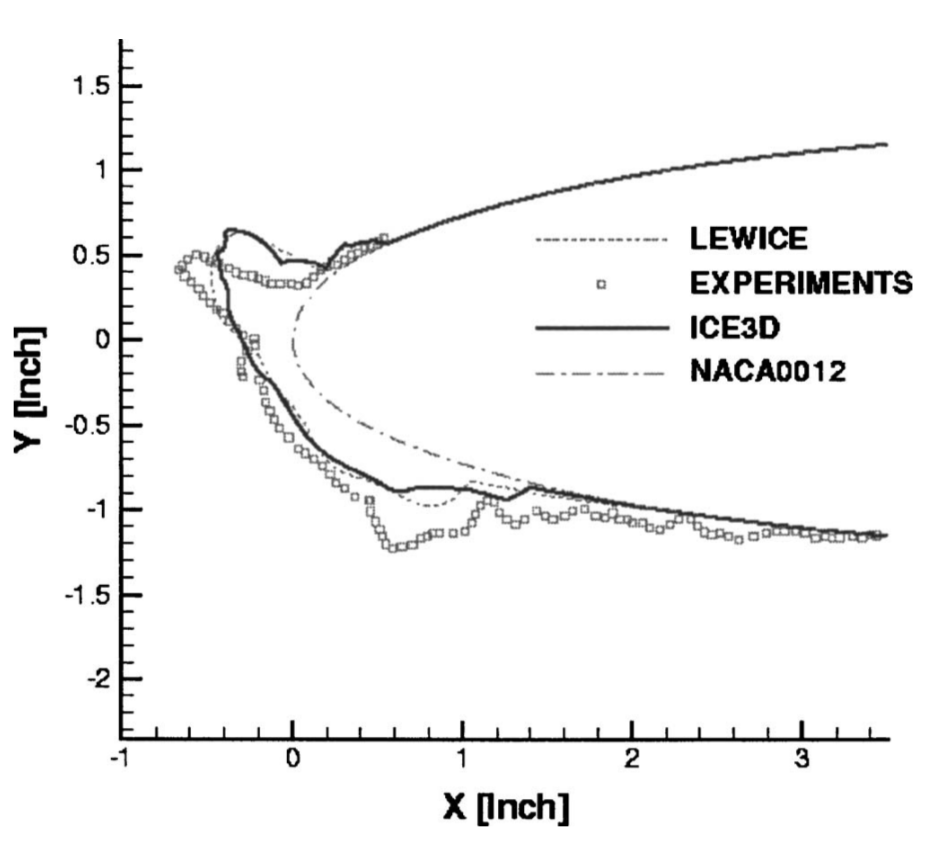
\includegraphics[width=0.4\textwidth]{Habashi2006ShapeVariation}}
      \subfigure[Wright, 2004]{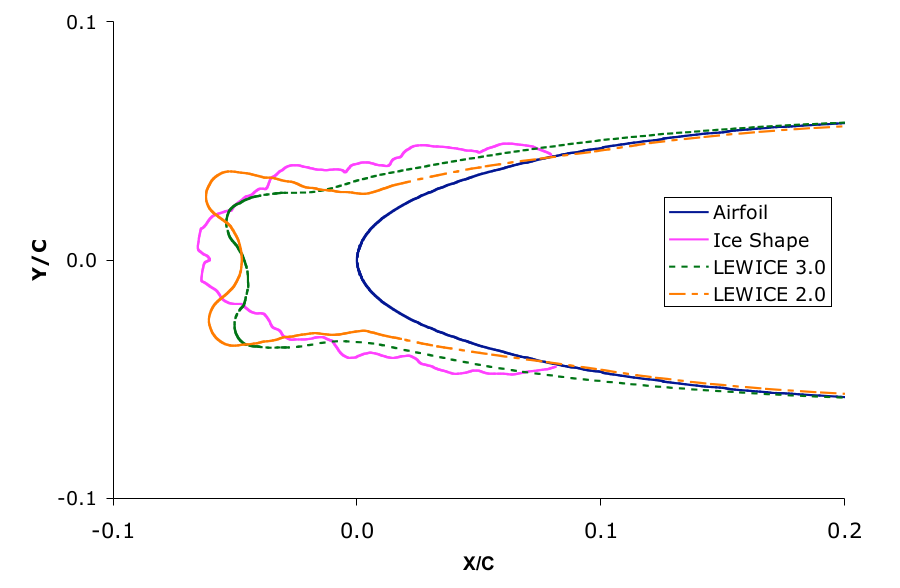
\includegraphics[width=0.4\textwidth]{Wright2004ShapeVariation}}
  \end{subfigmatrix}
\end{figure}

\begin{itemize}
\item Wide variation in experimental/computational ice shapes\footnote{Beaugendre H., Morency M., and Habashi W.G. \emph{Development of a Second Generation in-Flight Icing Simulation Code}. Journal of
Fluids Engineering, ASME, 2006.
 }\textsuperscript{,}\,\footnote{Wright W. and Potapczuk, M.G. \emph{Semi-Empirical Modeling of SLD Physics}, AIAA 2004-412. 42$^{nd}$ AIAA Aerospace Sciences
Meeting, Reno, NV, 2004.
 }
\item Suggests sensitivity to perturbations in underlying physical
  processes
\item \emph{UQ approach:} parameterize the shape variation and study its
  effects on aerodynamics
\end{itemize}
\end{frame}
\begin{frame}
\frametitle{Previous Work: Heuristic UQ}
\label{sec-1-3}


\begin{columns}[c]
  \column{0.33\textwidth}
    \centering
    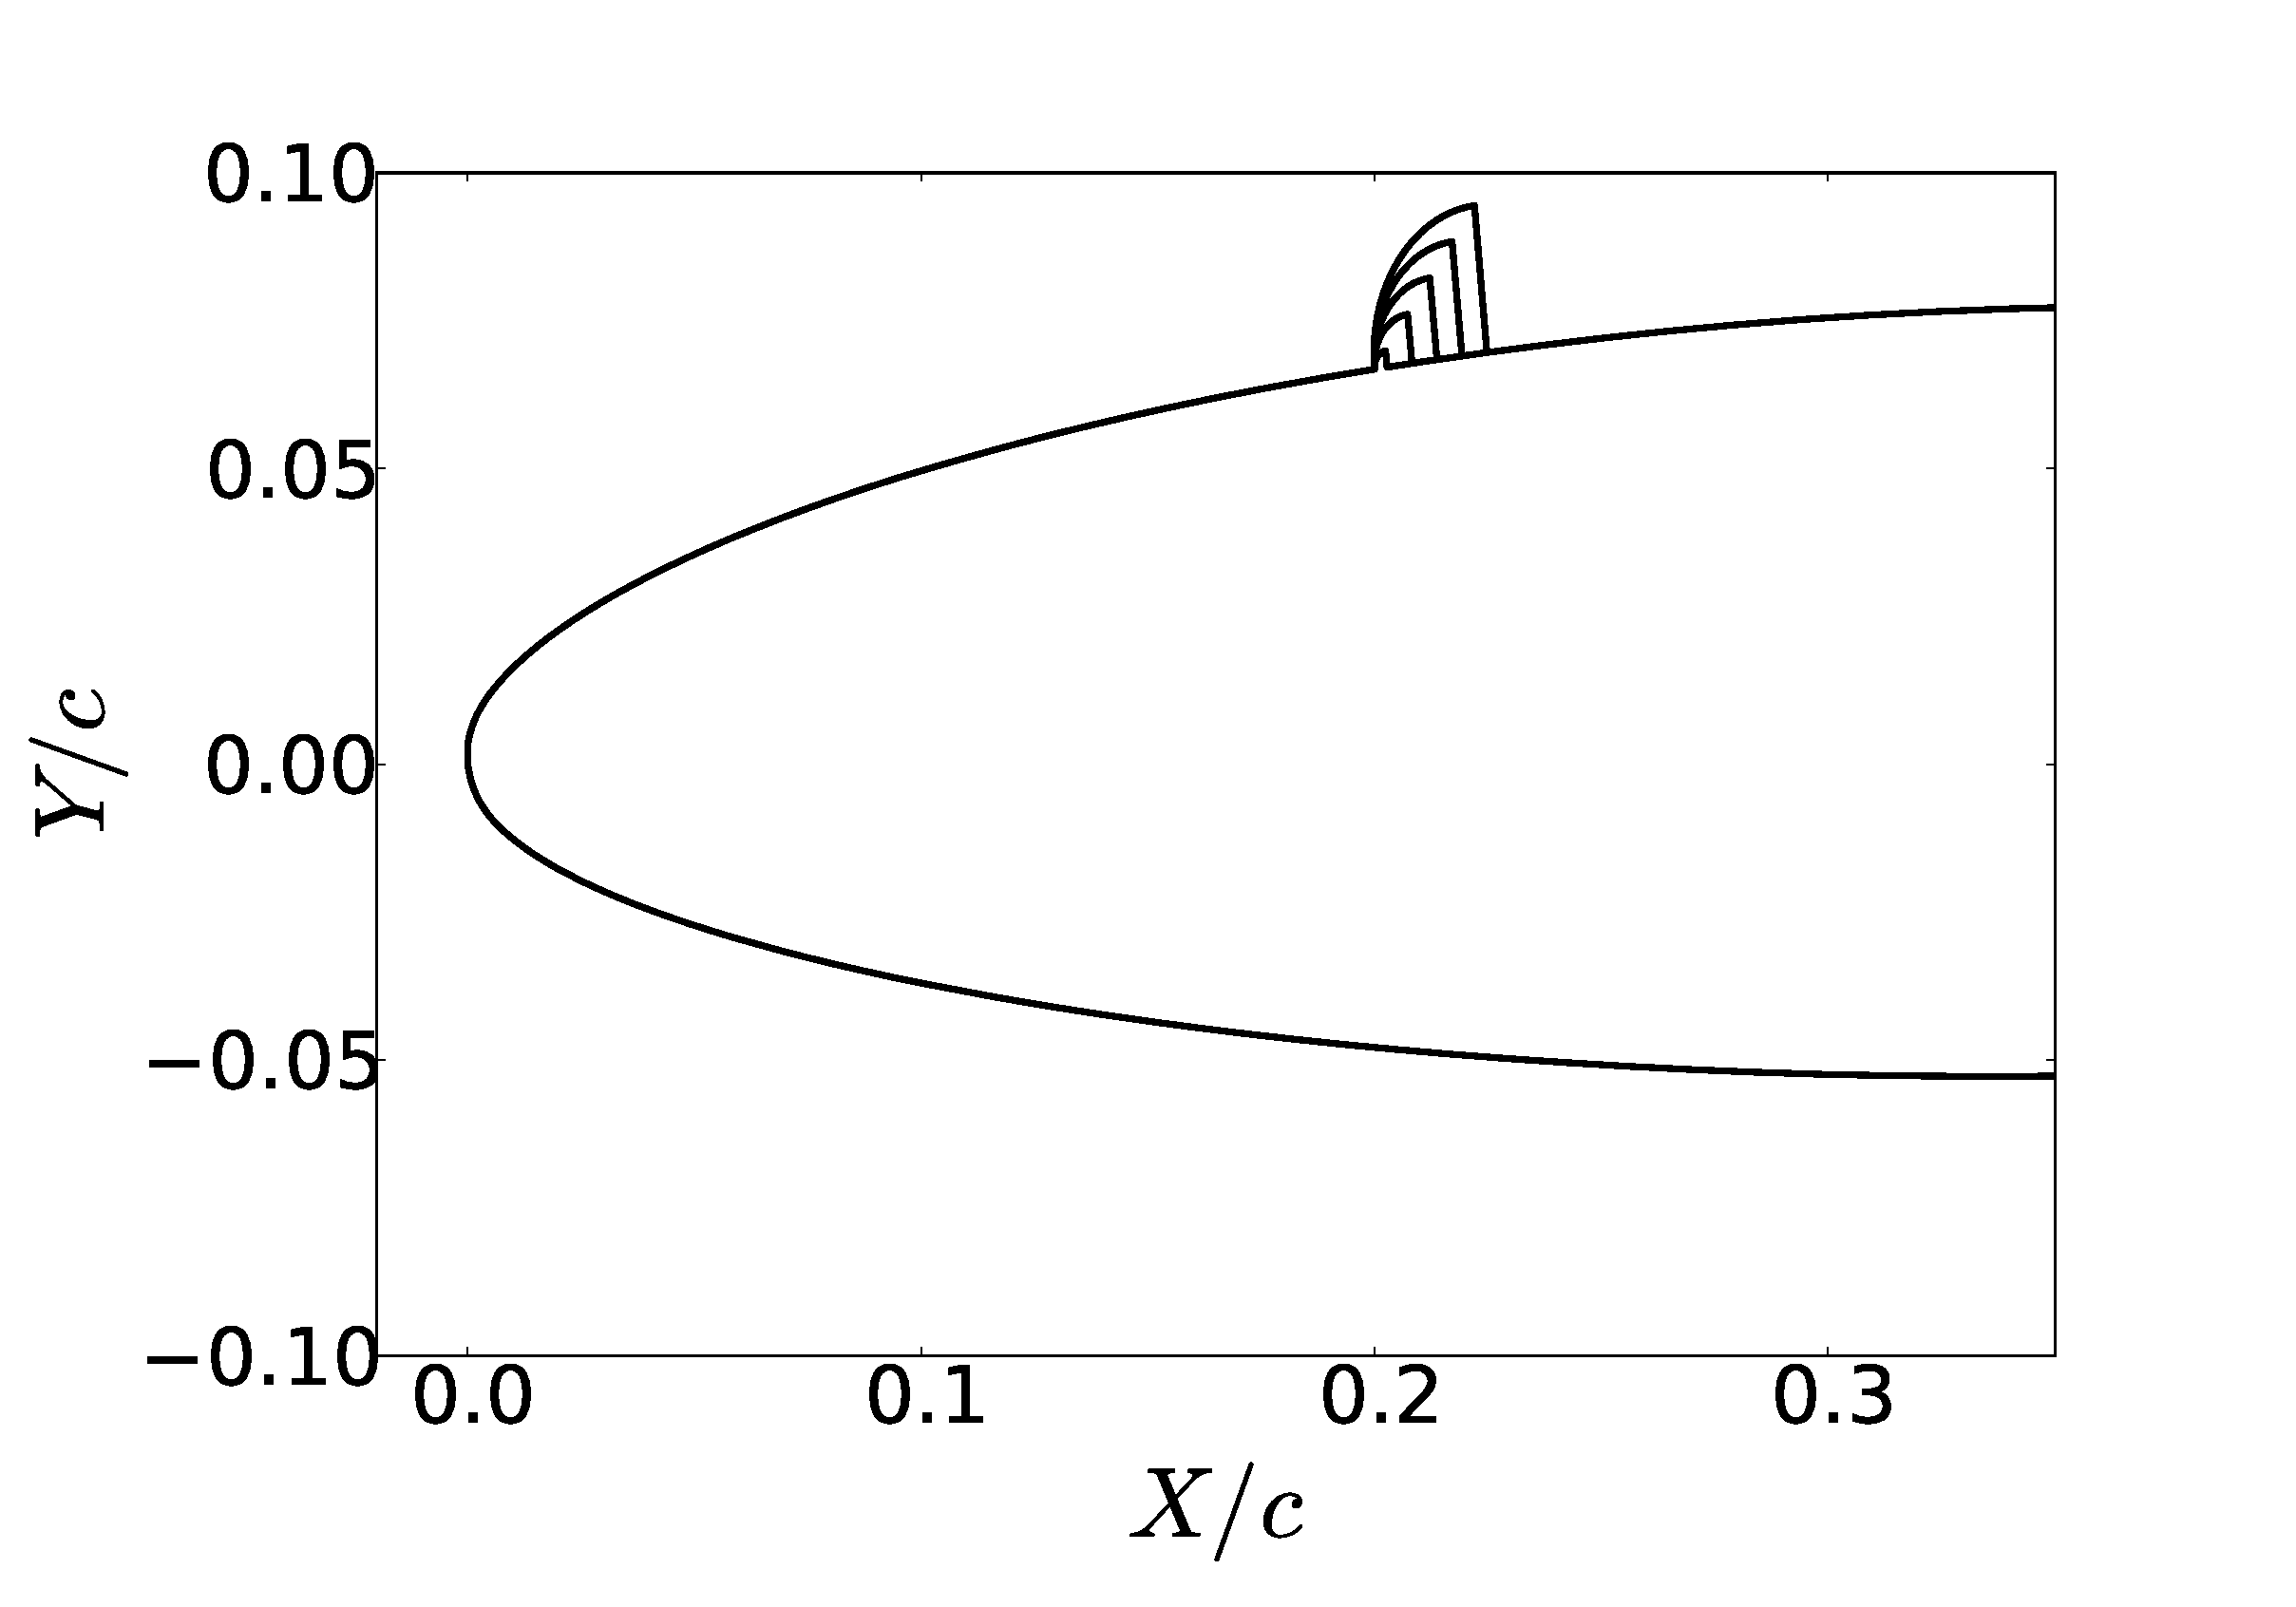
\includegraphics[width=0.95\textwidth]{RidgeRVariation} \\
    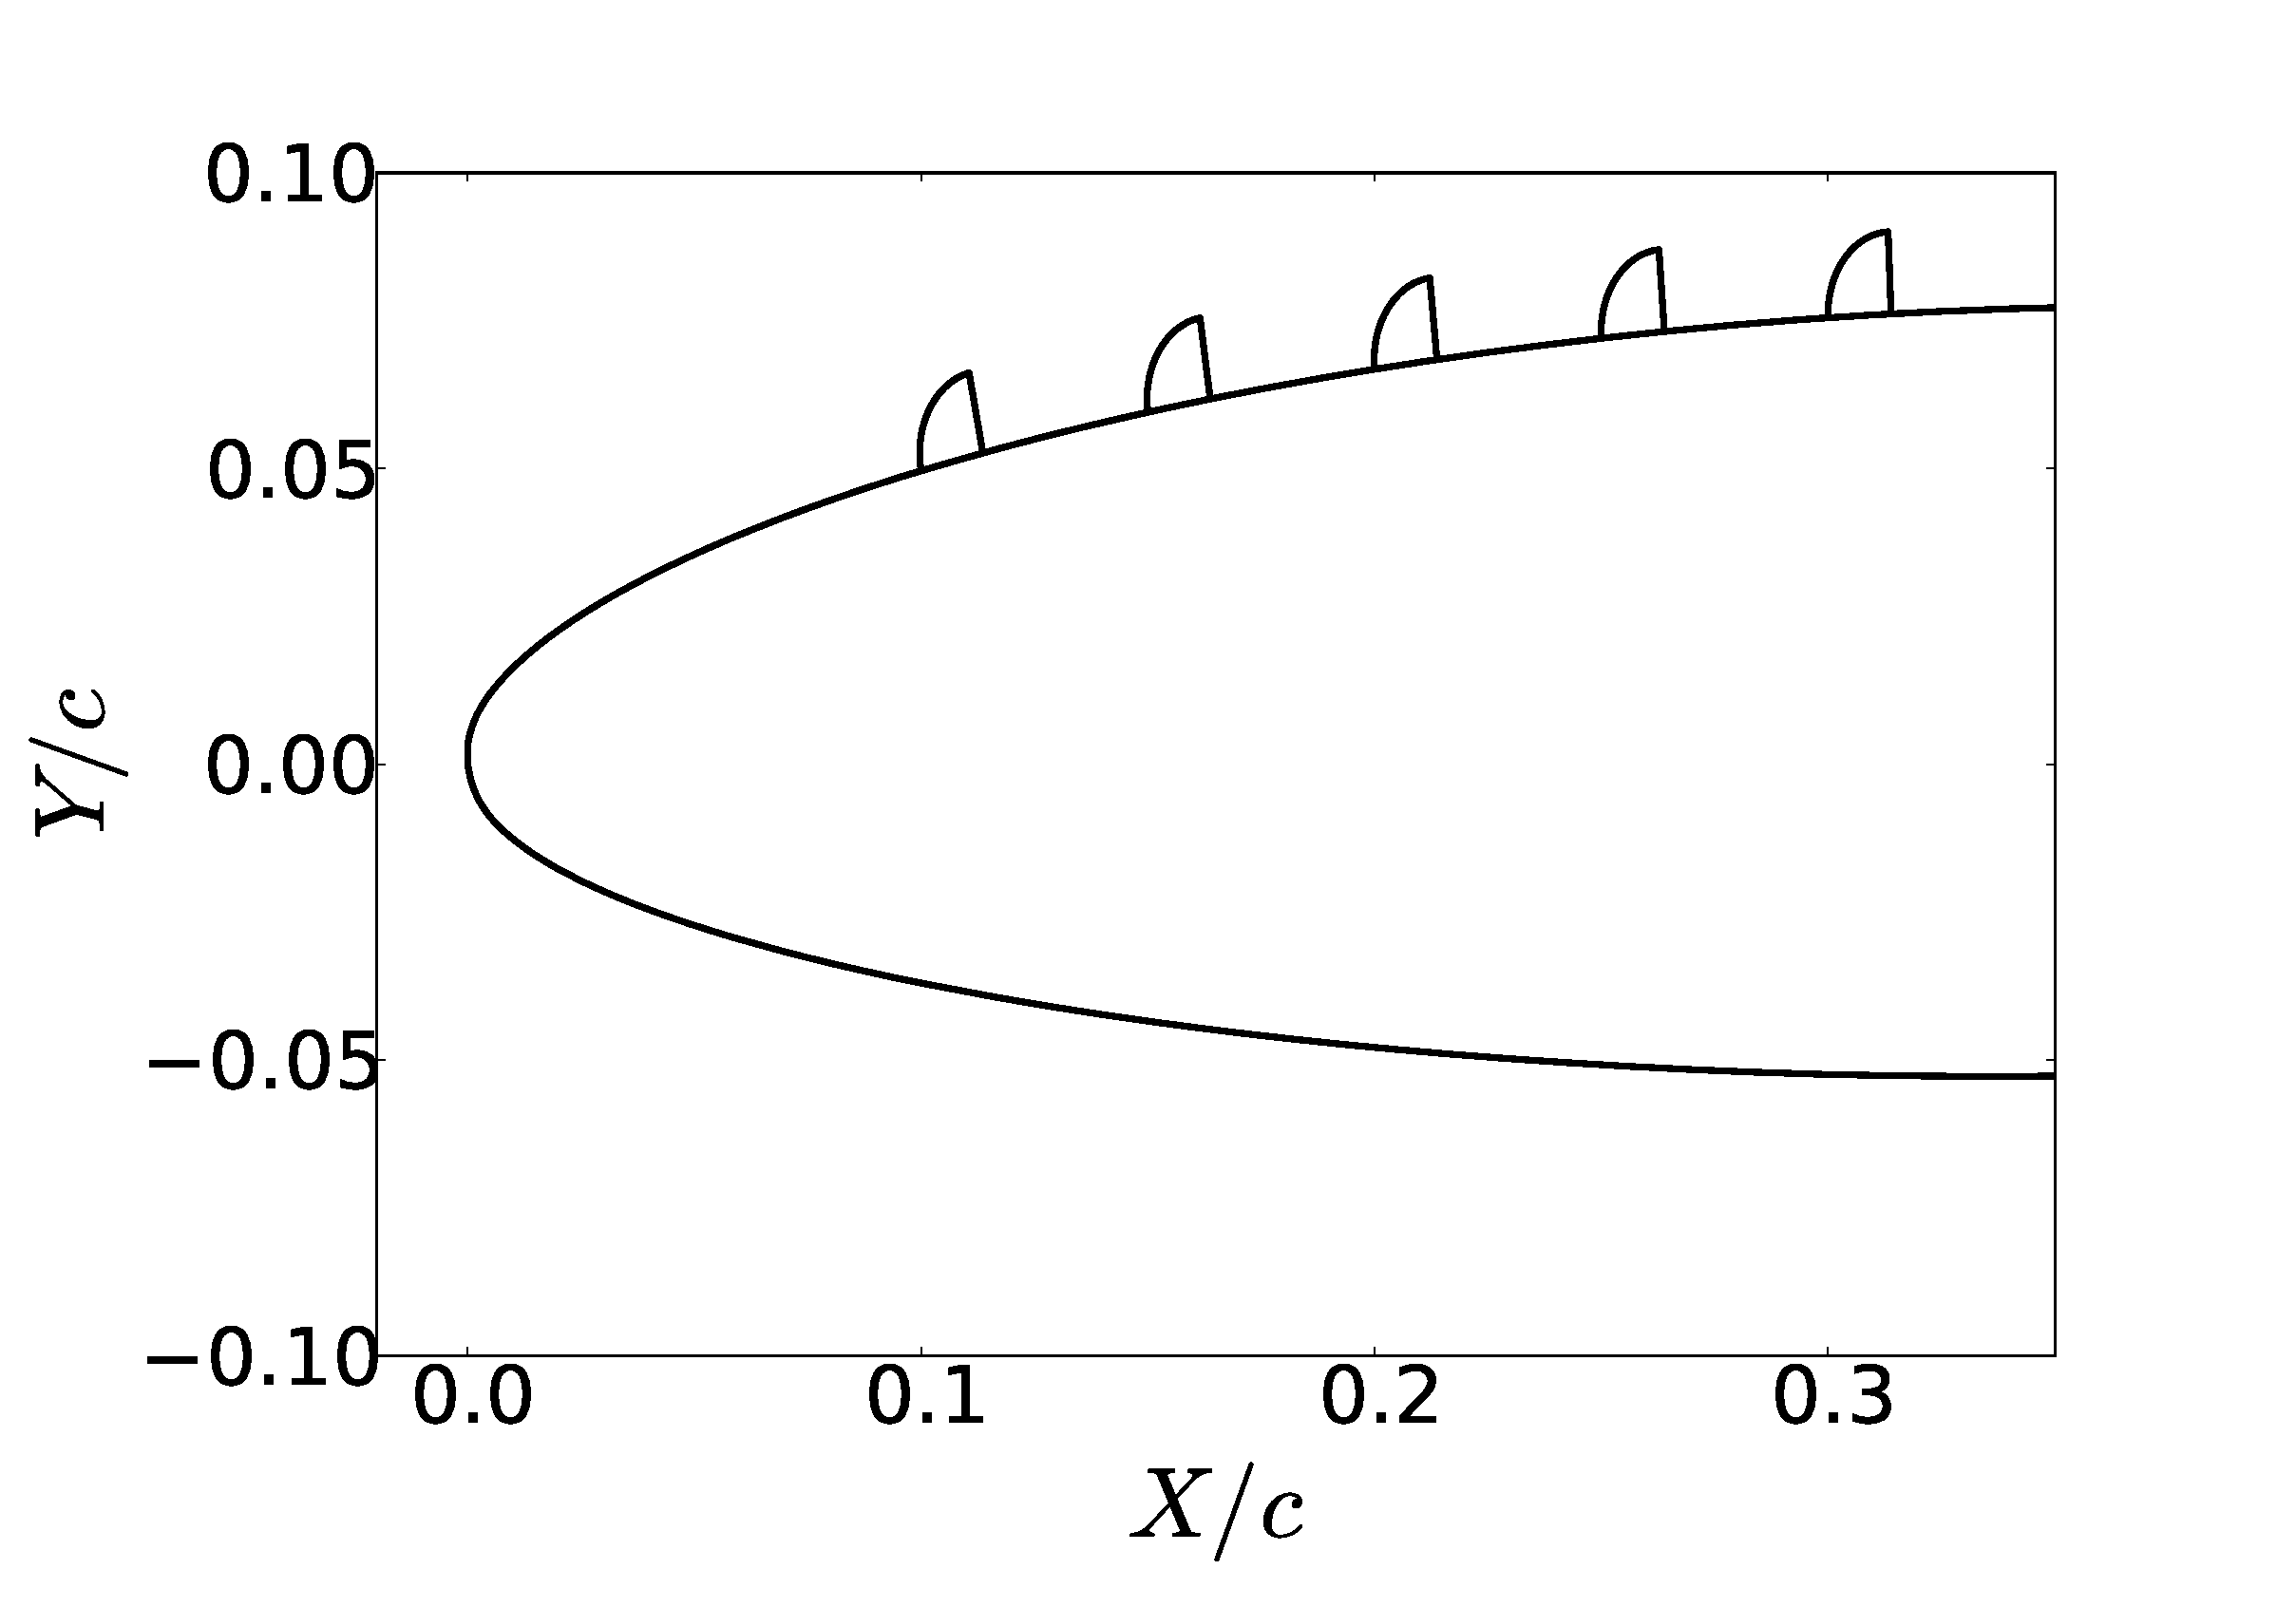
\includegraphics[width=0.95\textwidth]{RidgeSVariation} \\
    {\bf Ridge}
  \column{0.33\textwidth}
    \centering
    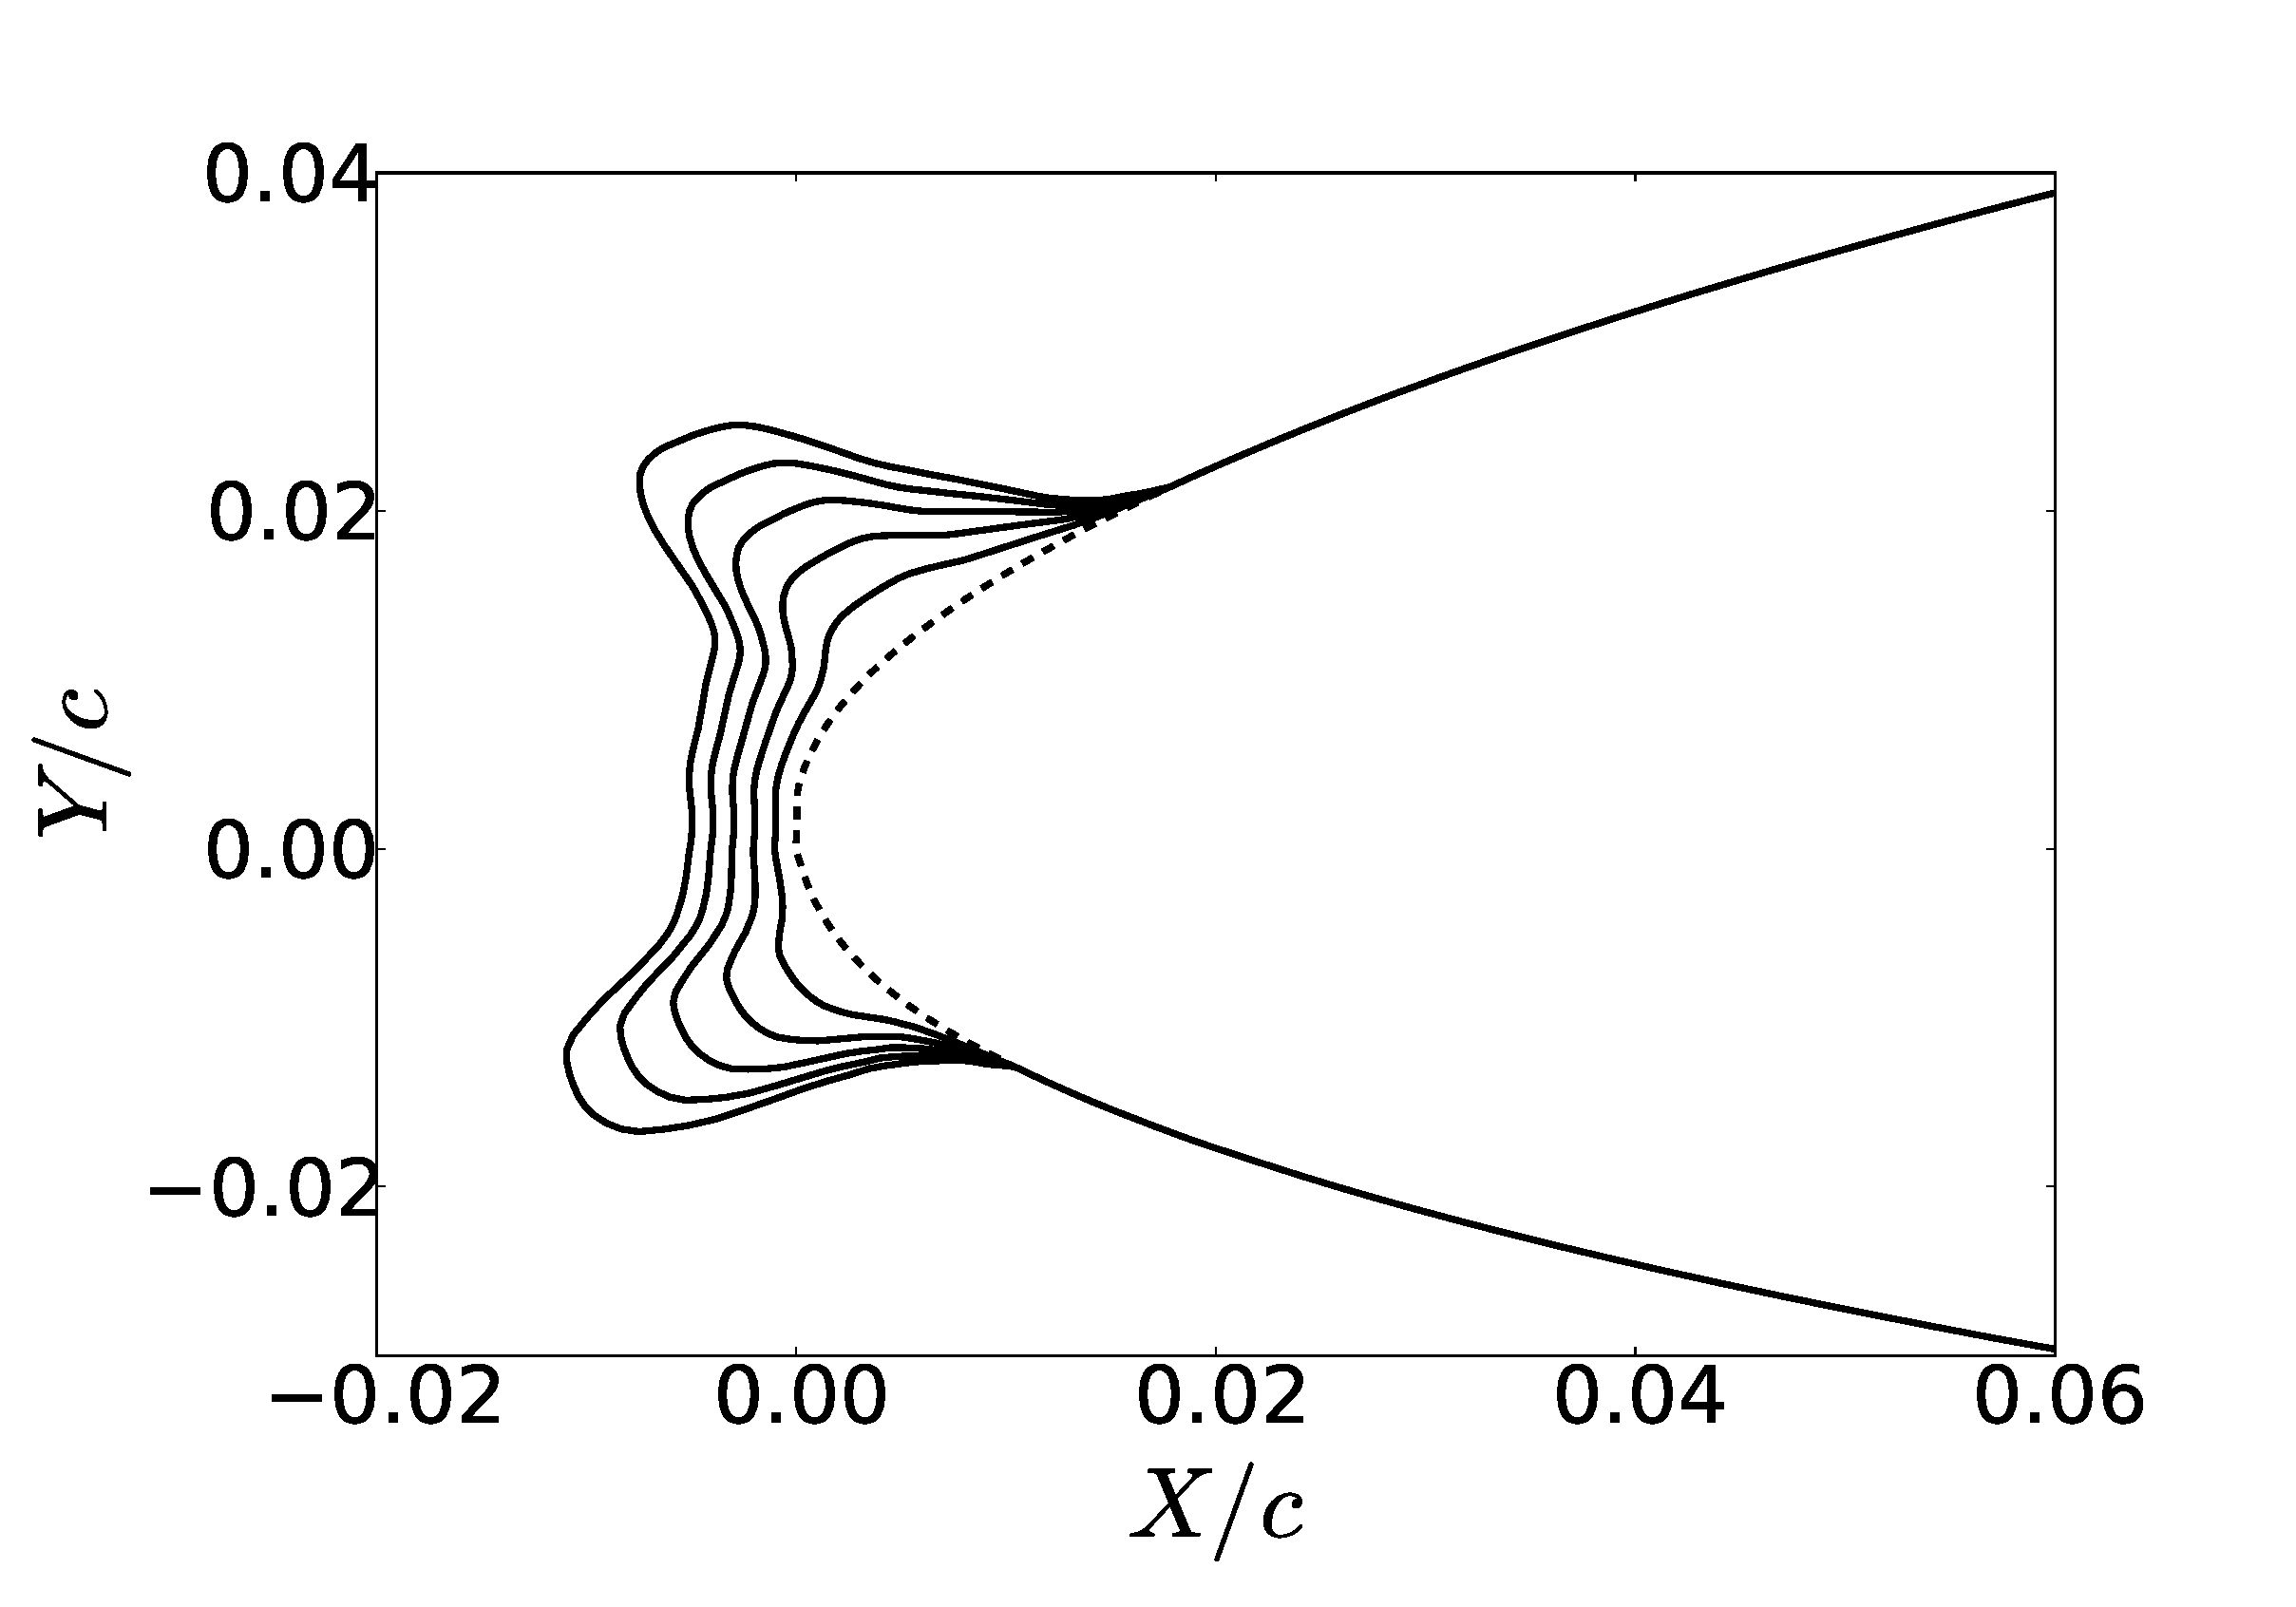
\includegraphics[width=0.95\textwidth]{HornHVariation} \\
    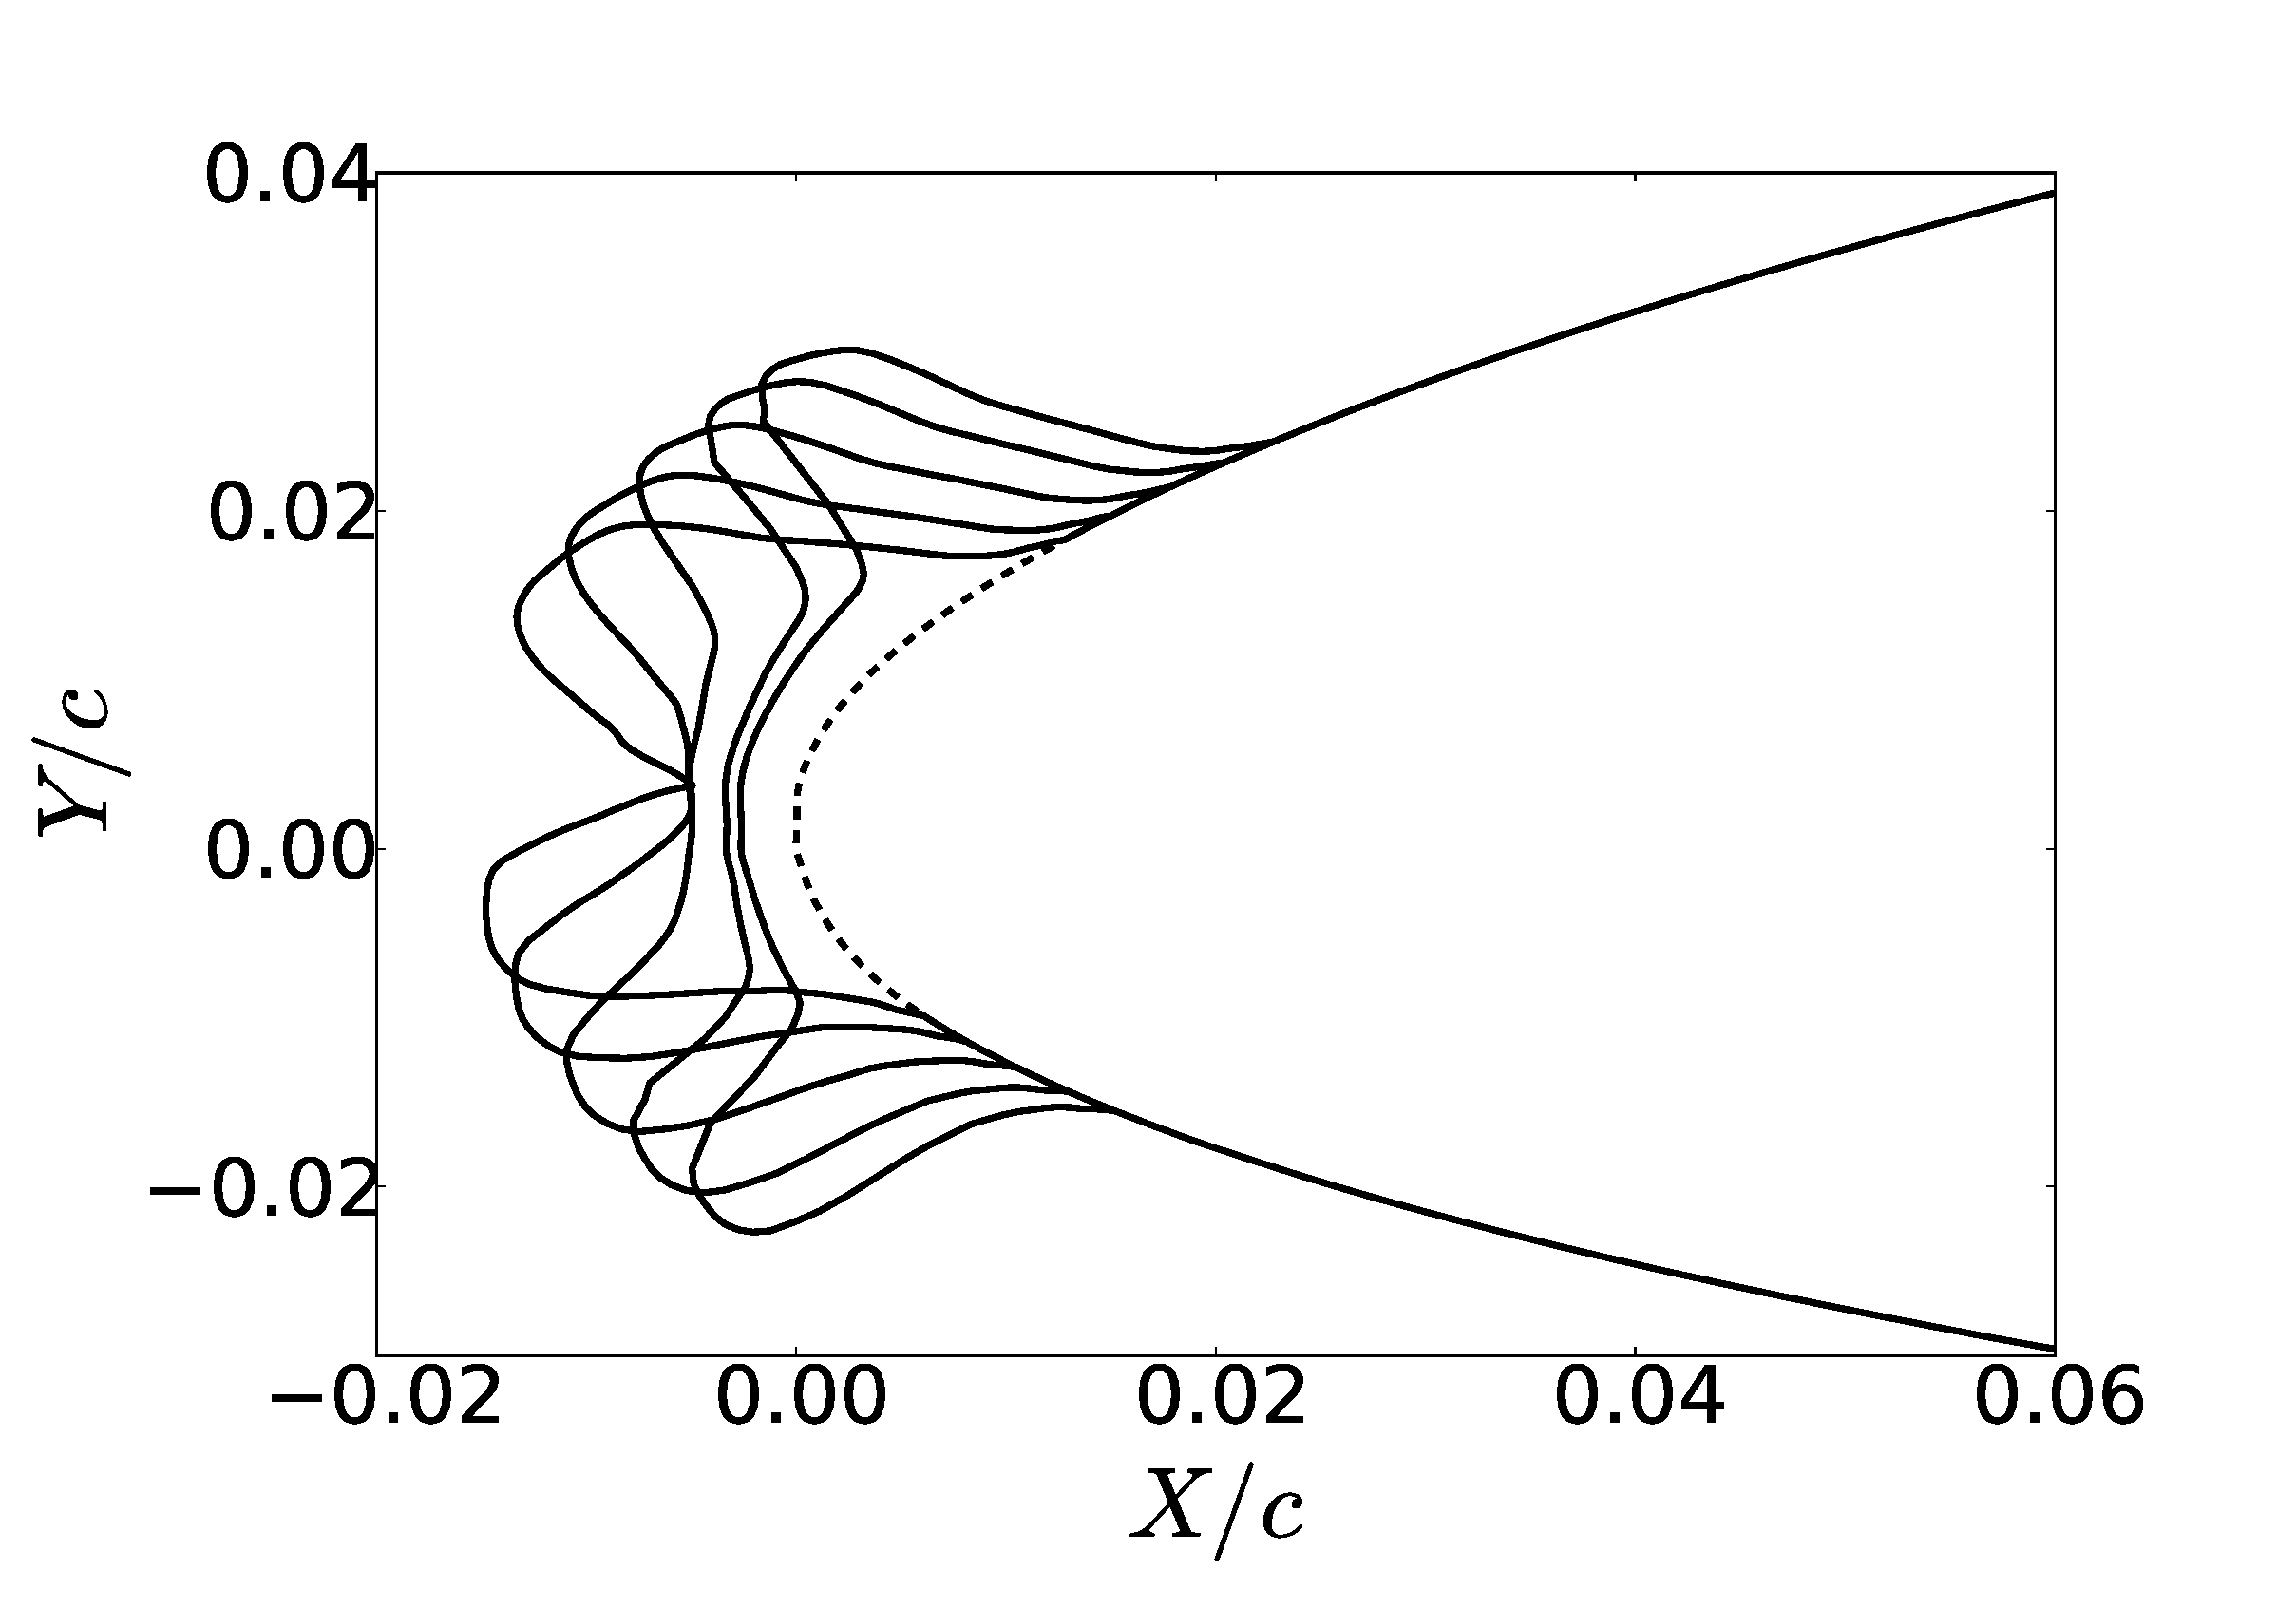
\includegraphics[width=0.95\textwidth]{HornSVariation} \\
    {\bf Horn}
  \column{0.33\textwidth}
    \centering    
    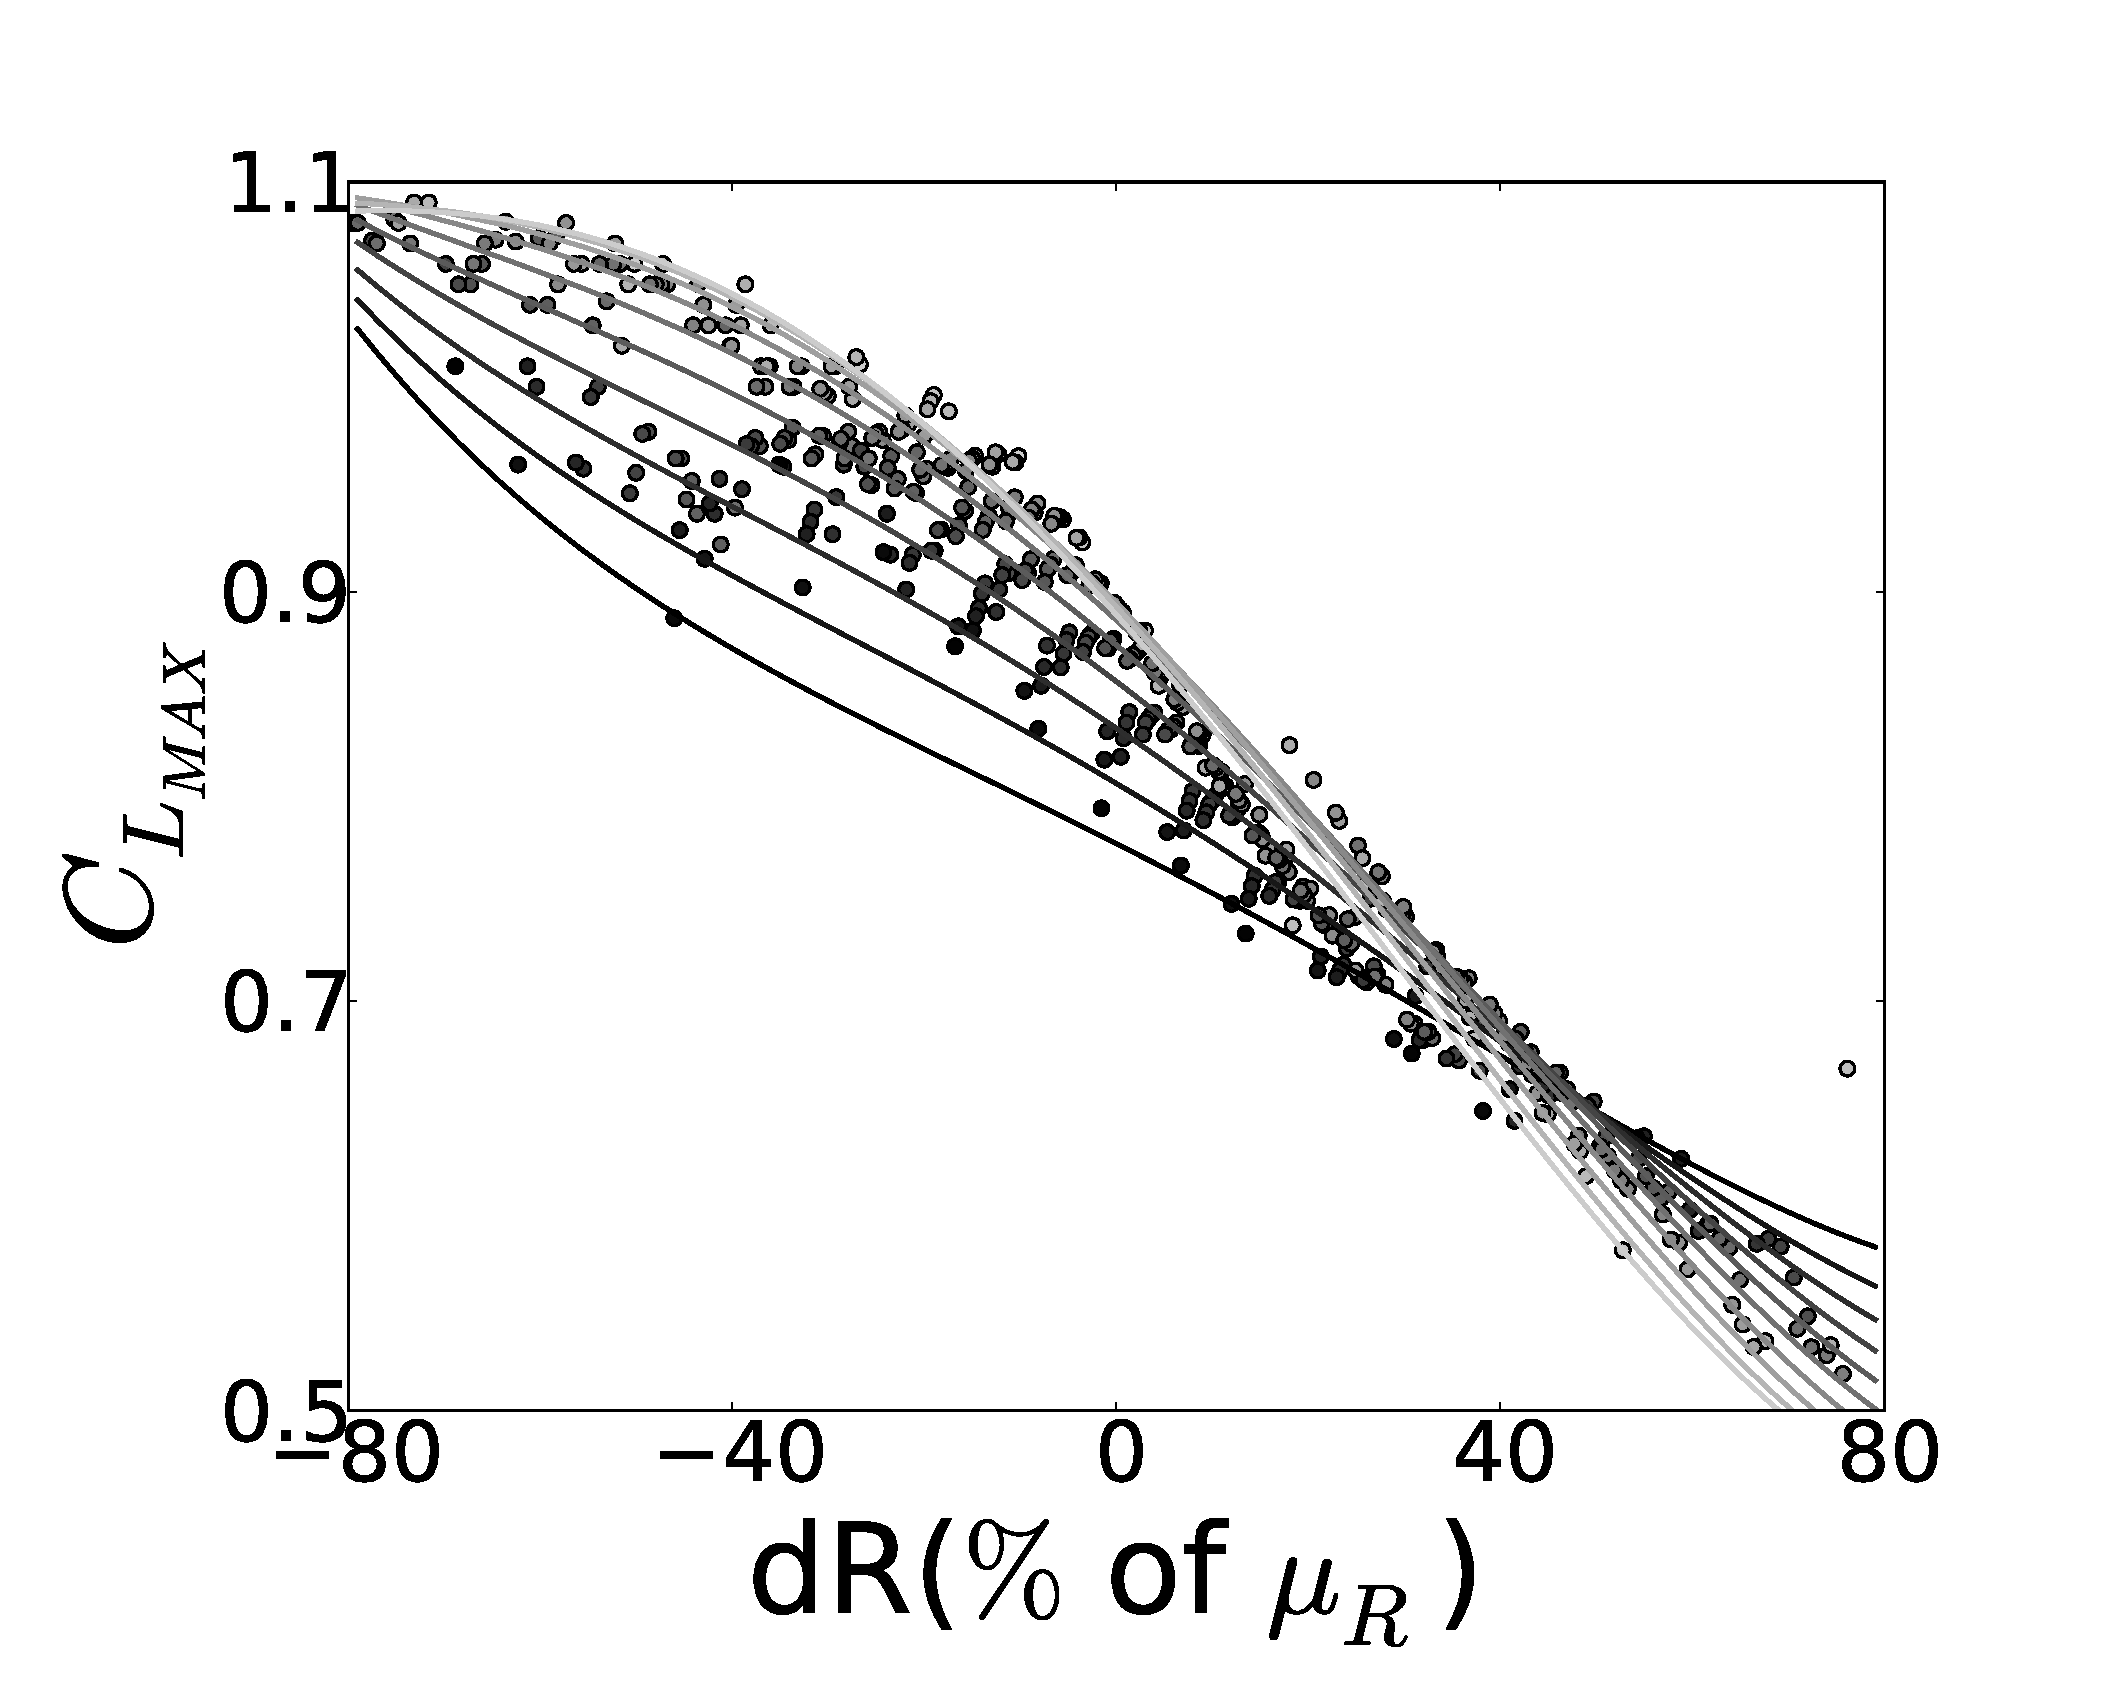
\includegraphics[width=0.9\textwidth]{MC_surrogate_LargeUnc_CL} \\
    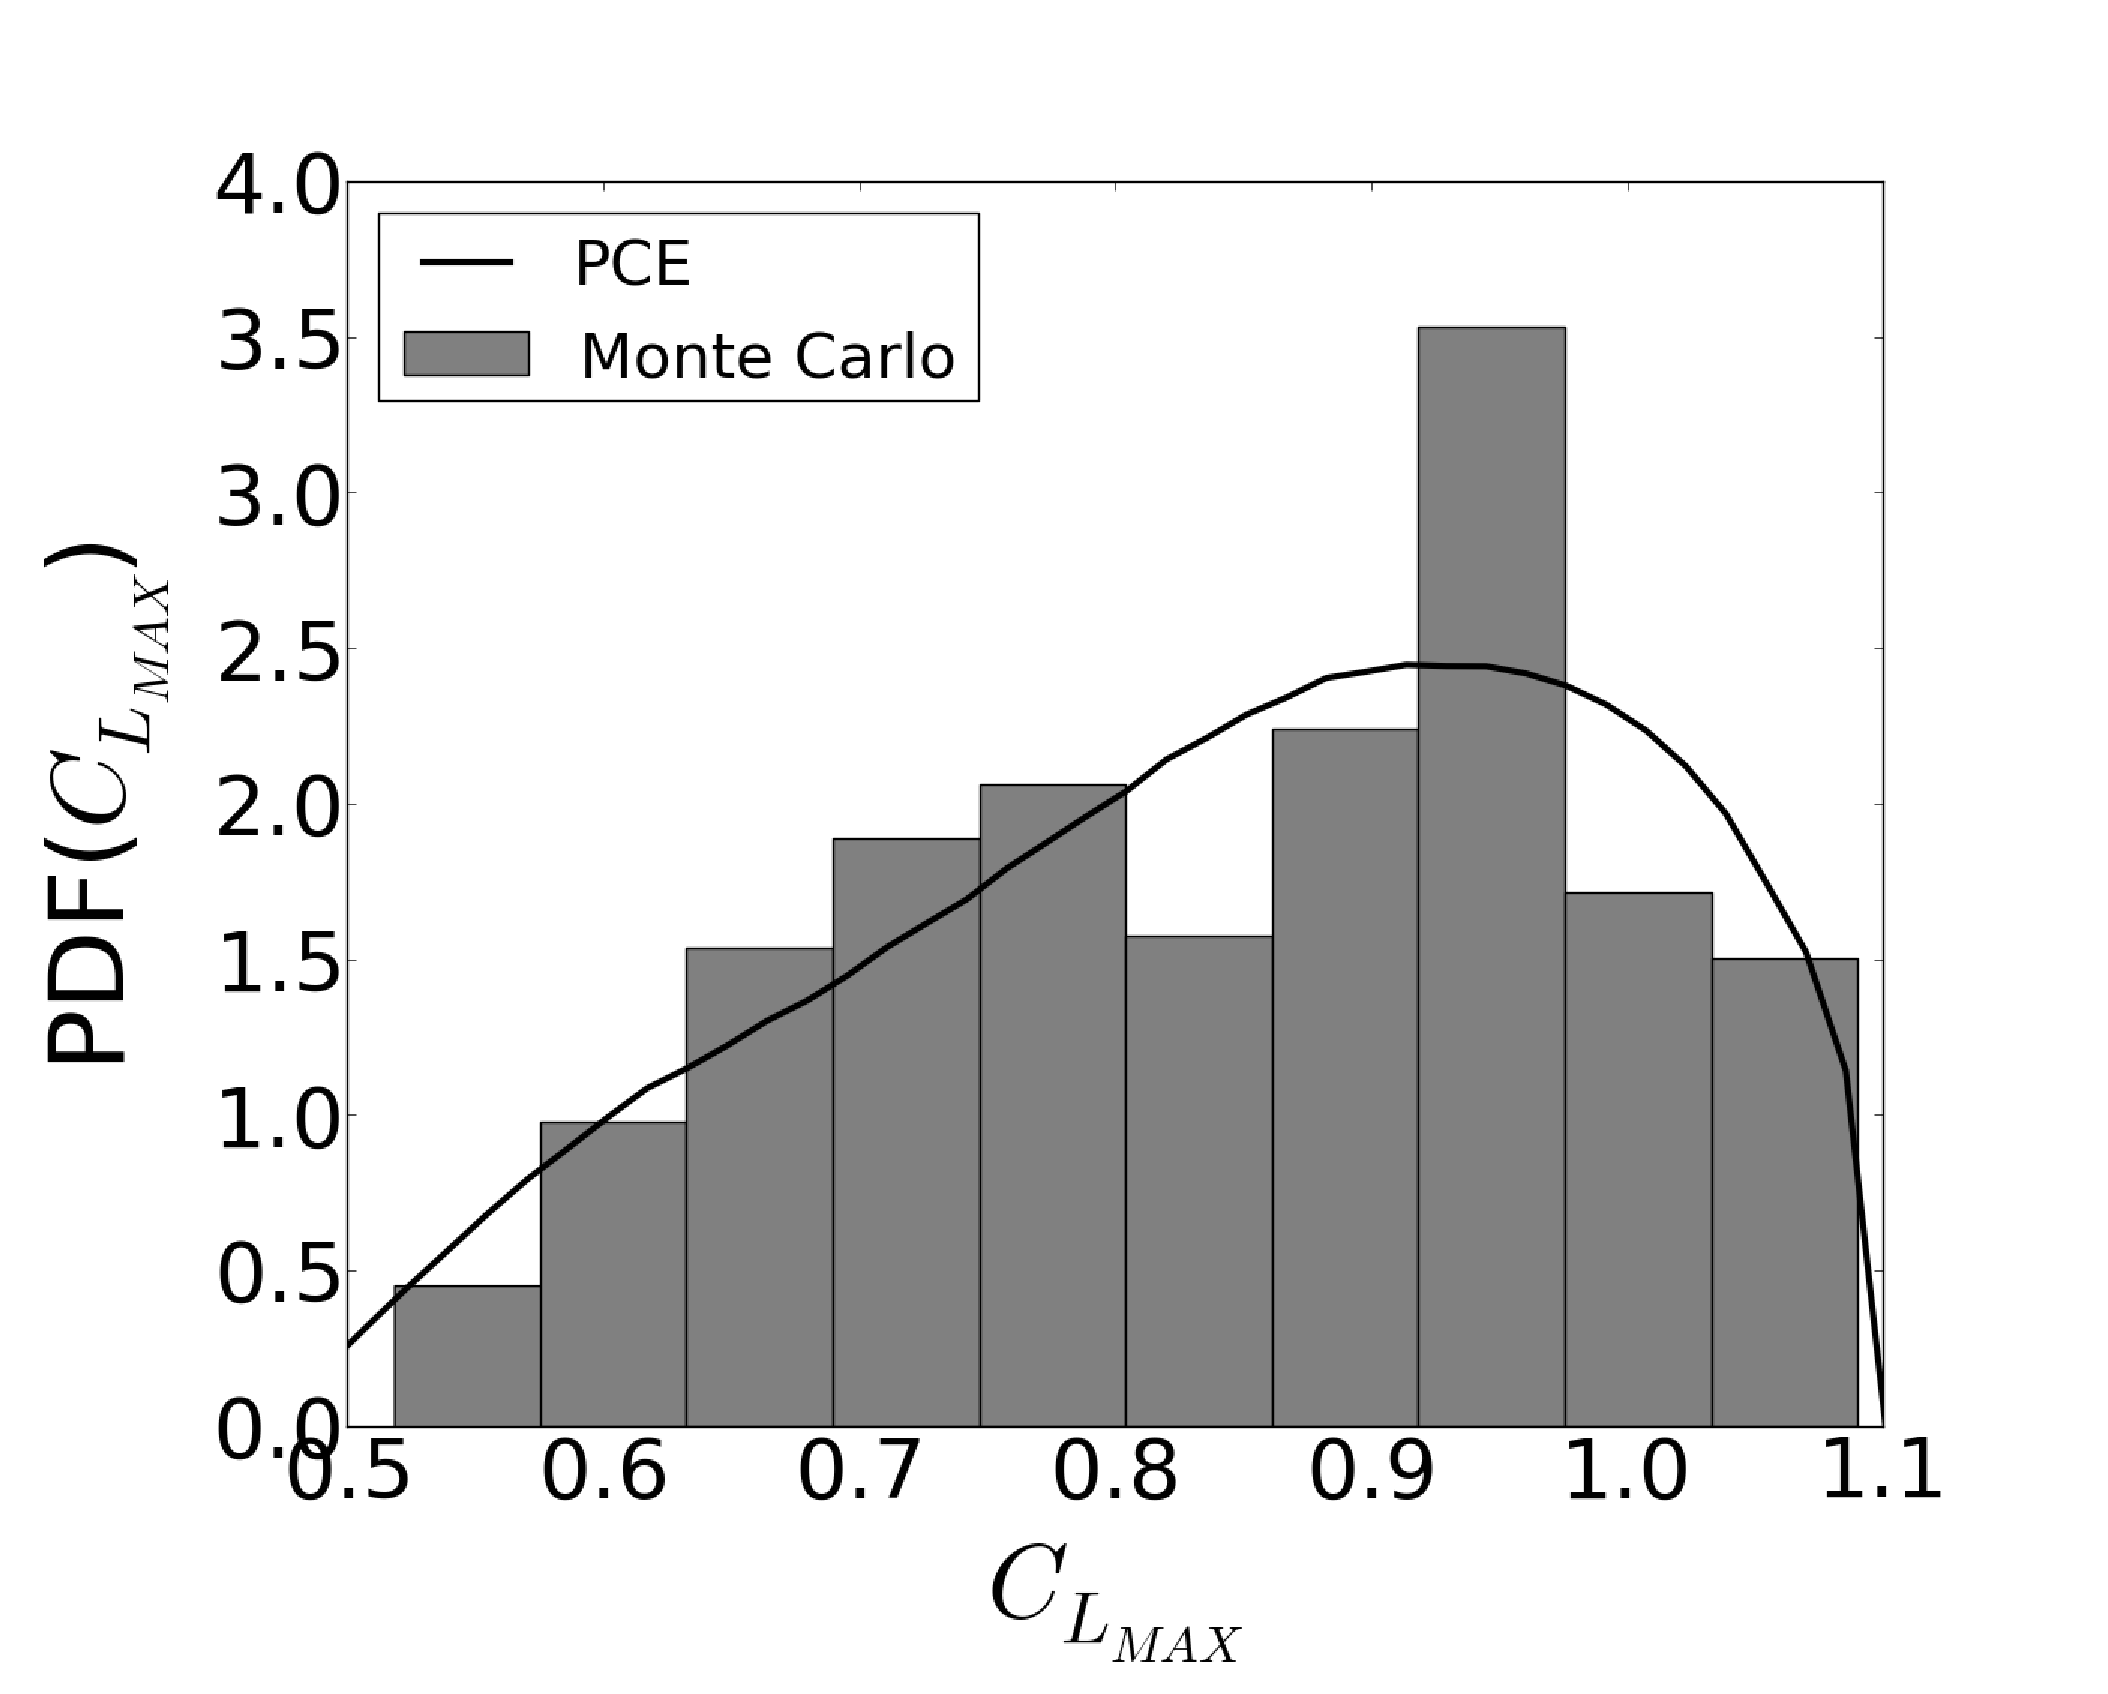
\includegraphics[width=0.9\textwidth]{MCgpcPDFLargeUnc_CL} \\
    {\bf Statistics}
\end{columns}

\begin{itemize}
\item Previous study examined parameterized ridge and horn ice
  shapes\footnote{DeGennaro A., Rowley C.W., and Martinelli,
L. \emph{Uncertainty Quantification for Airfoil Icing using Polynomial Chaos Expansions}. Journal of Aircraft, 2015.
 }
\item Approach was heuristic, not directly based on observed shape
  variations
\item Parameter space was low dimensional; no low-dimensional modeling
\end{itemize}
\end{frame}
\begin{frame}
\frametitle{Previous Work: Data-Driven UQ}
\label{sec-1-4}

\begin{figure}
  \centering
  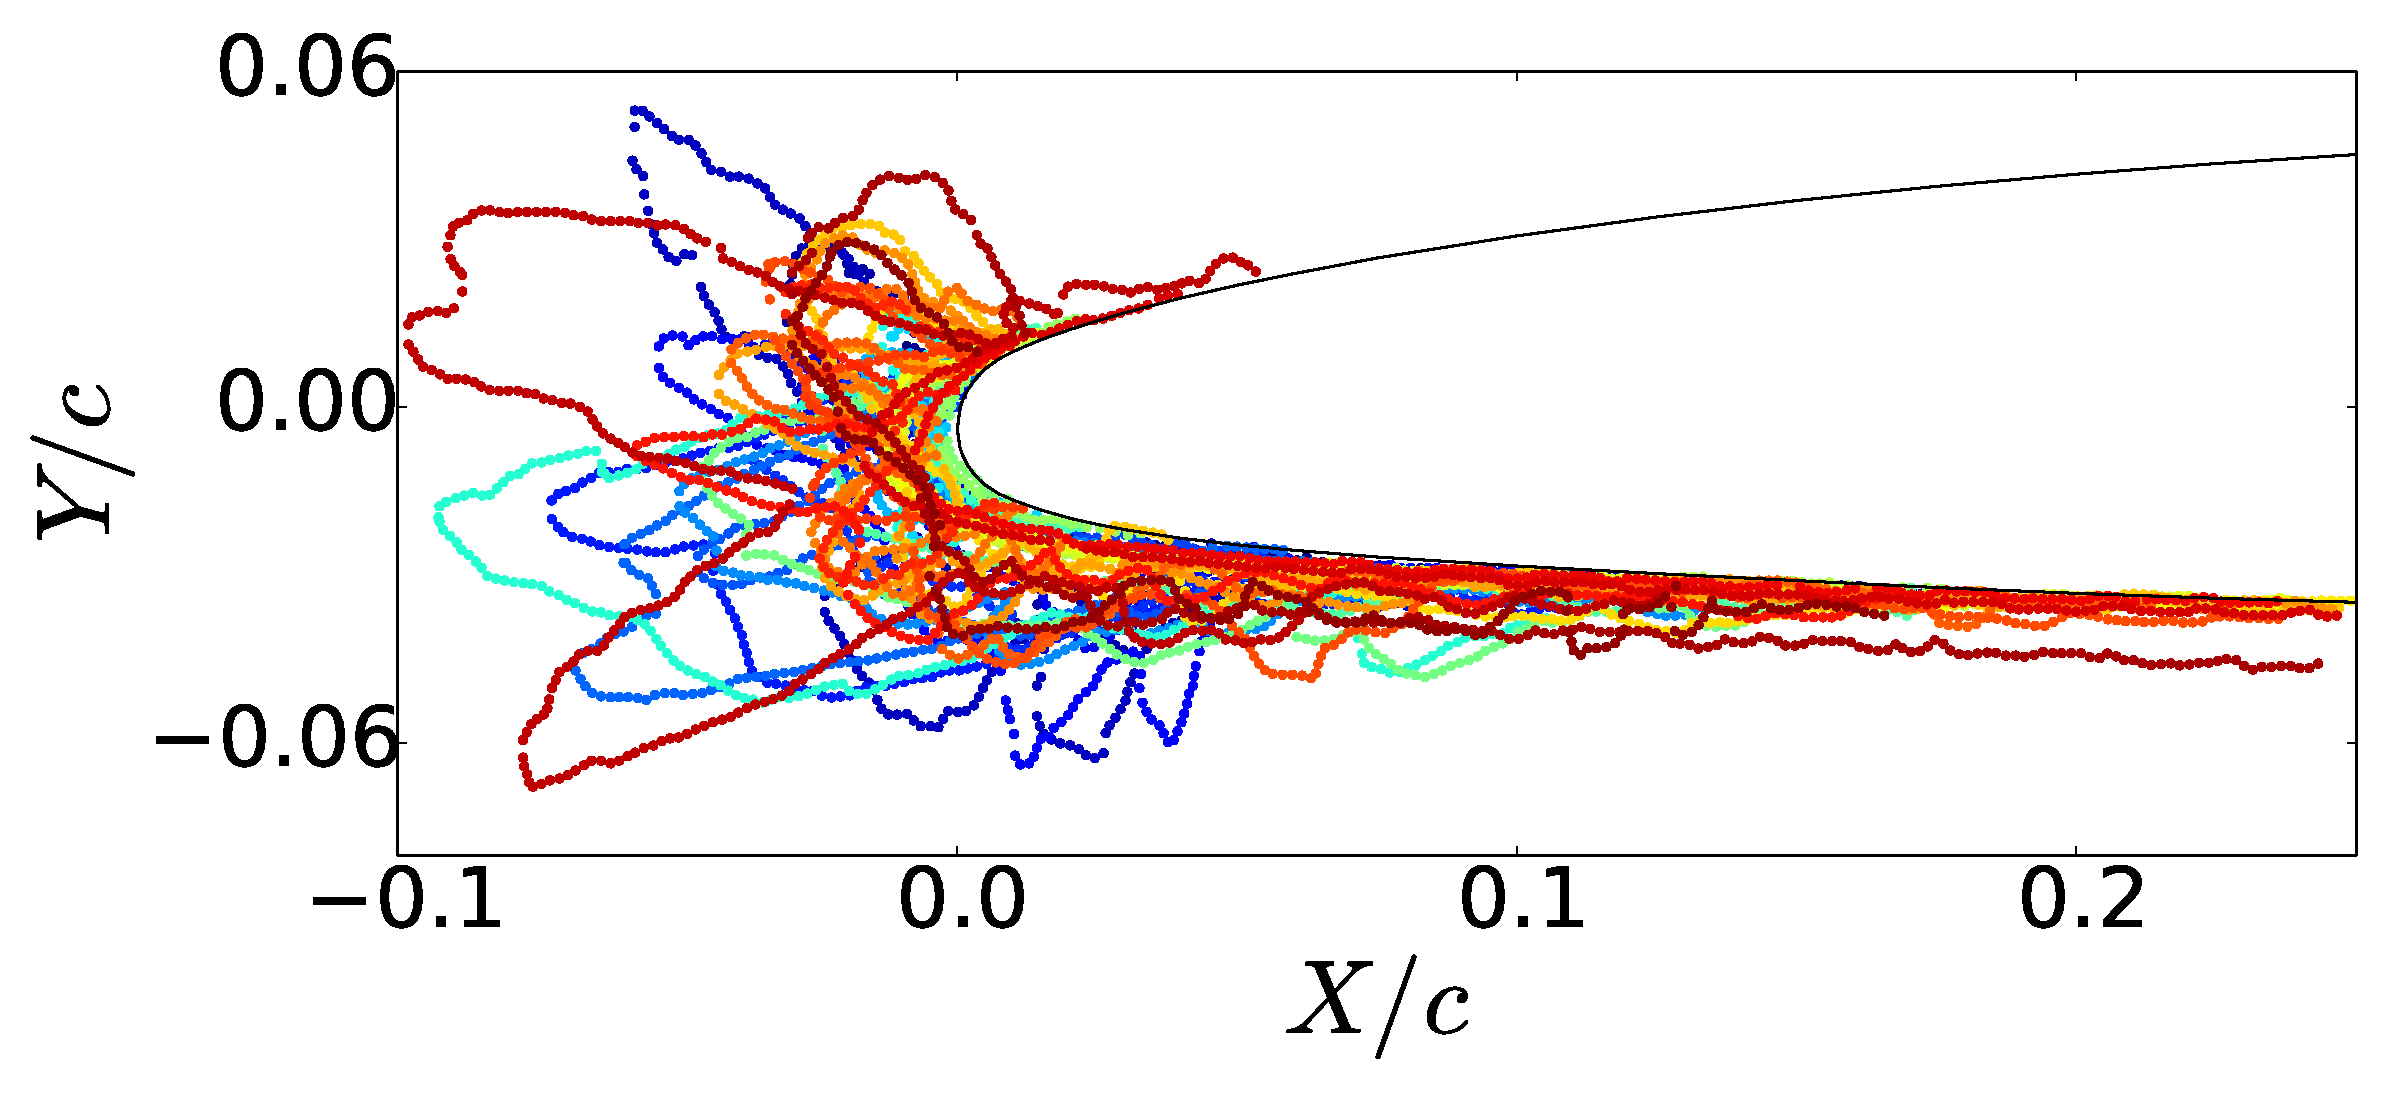
\includegraphics[width=0.7\textwidth]{Dataset}
\end{figure}

\begin{itemize}
\item \textbf{Select a database of ice shapes}
\begin{itemize}
\item 54 ice shapes, exposed to a wide range of various icing conditions
    consistent with FAA certification guidelines\footnote{Addy, H.E. \emph{Ice Accretions and Icing Effects for Modern Airfoils}. NASA TR 2000-210031.
 }
\end{itemize}
\end{itemize}
\end{frame}
\begin{frame}
\frametitle{Previous Work: Data-Driven UQ}
\label{sec-1-5}

\begin{columns}[c]
  \column{0.45\textwidth}
    \centering
    \hspace{-2.17em}
    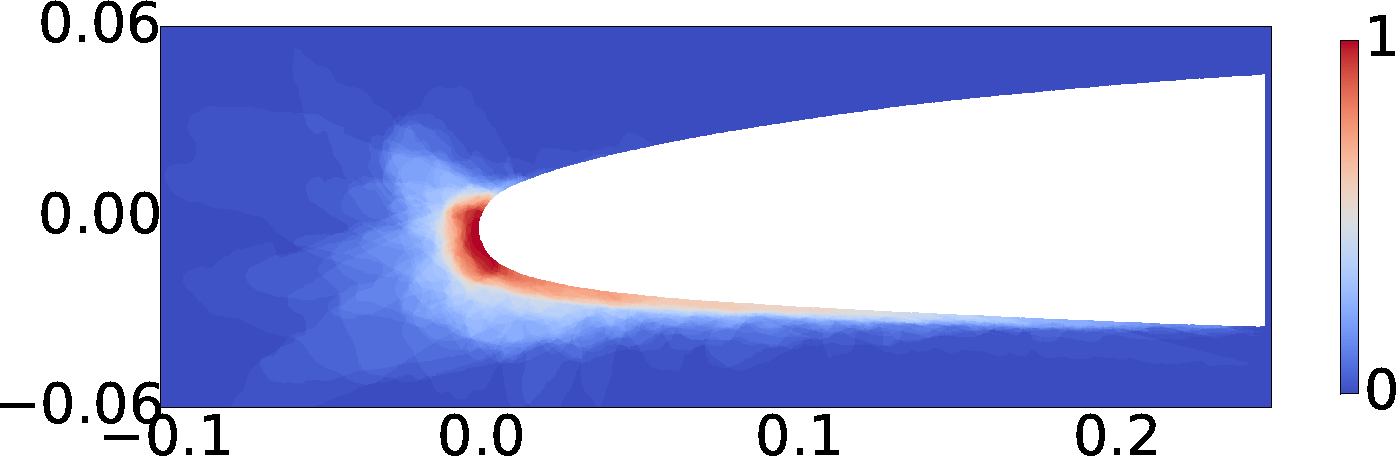
\includegraphics[width=0.9\textwidth]{MEAN.png} \\
    {\bf Mean} \\
    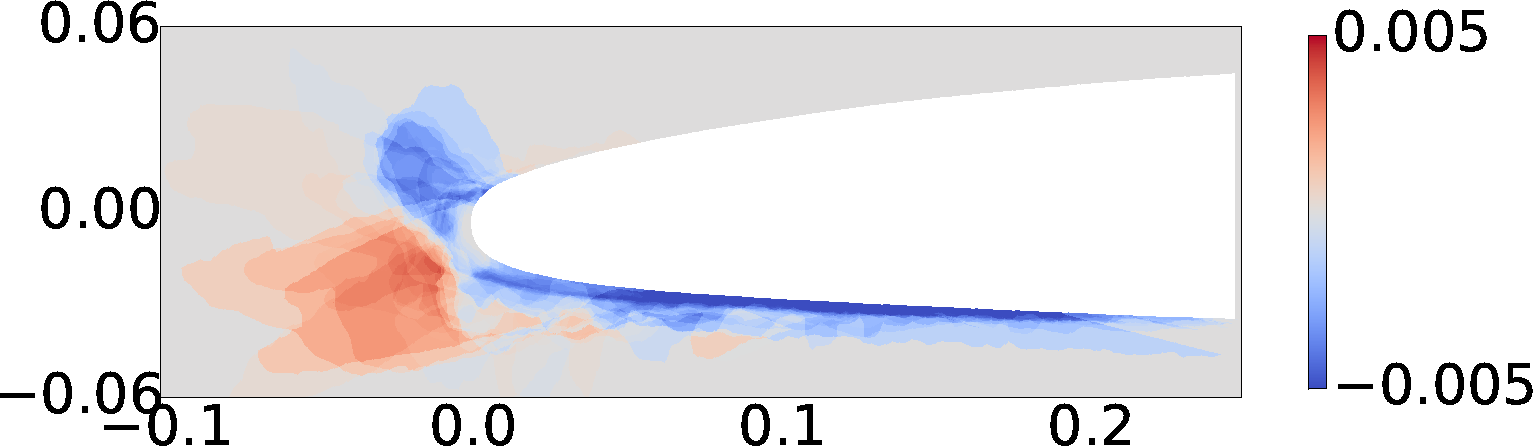
\includegraphics[width=1\textwidth]{MODE2.png} \\
    {\bf Mode 2} \\
    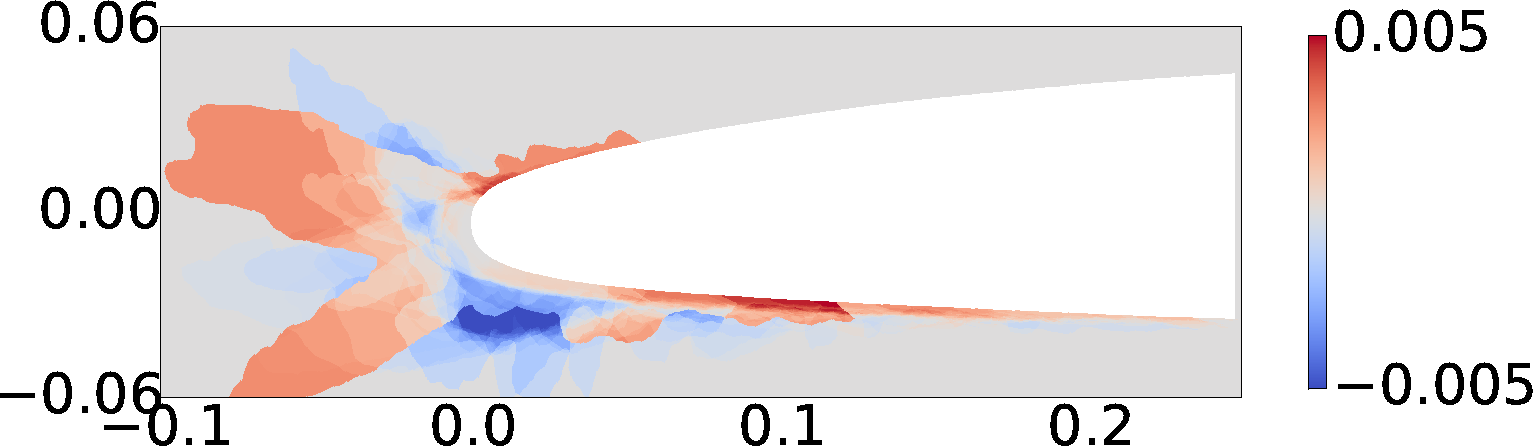
\includegraphics[width=1\textwidth]{MODE4.png} \\
    {\bf Mode 4}
  \column{0.45\textwidth}
    \centering
    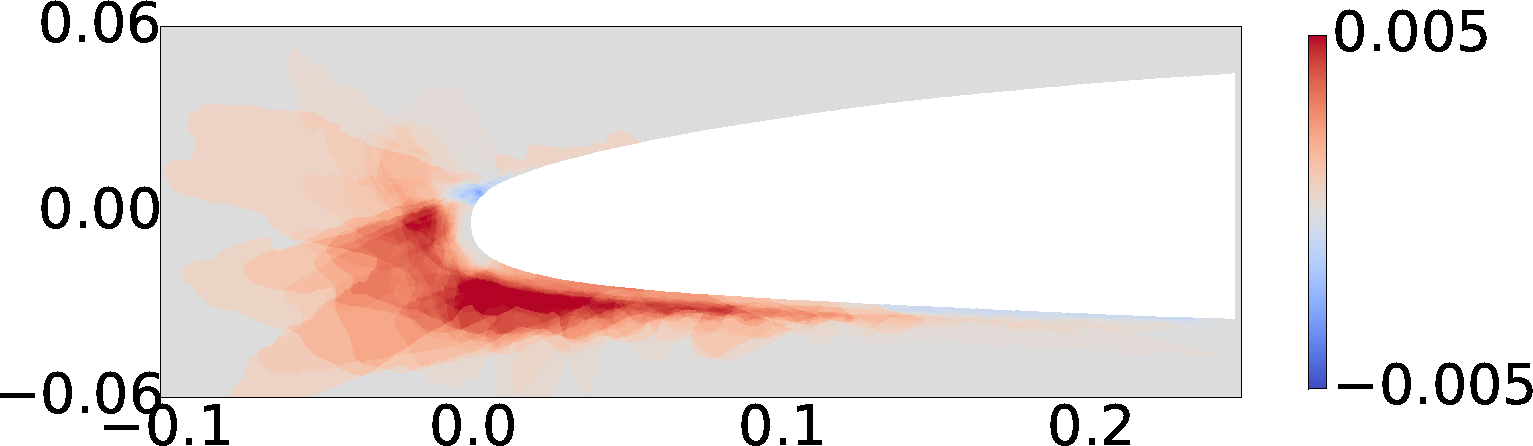
\includegraphics[width=1\textwidth]{MODE1.png} \\
    {\bf Mode 1} \\
    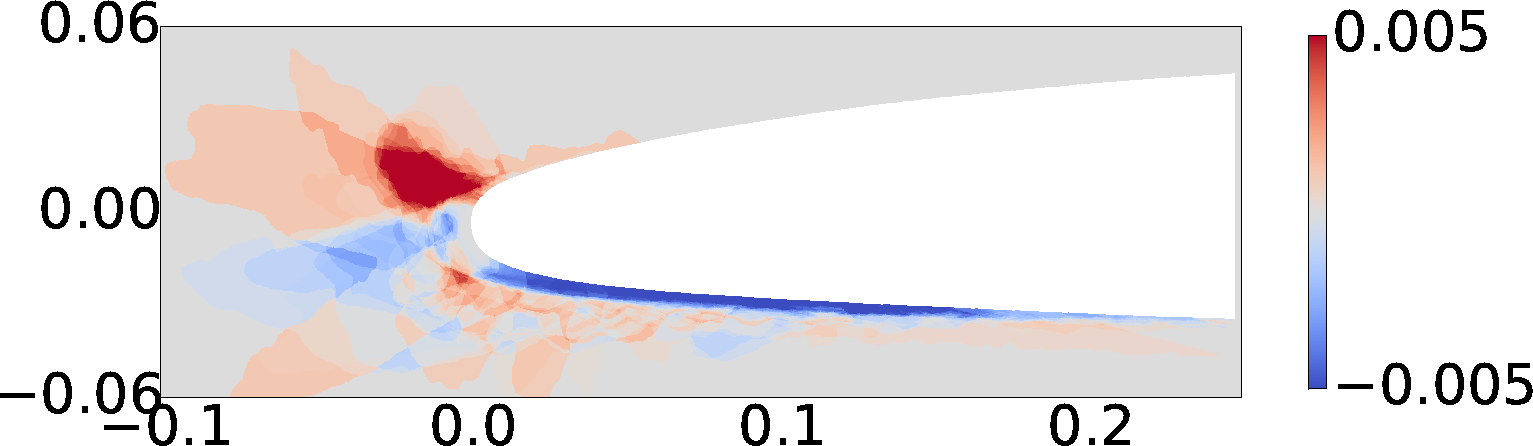
\includegraphics[width=1\textwidth]{MODE3.png} \\
    {\bf Mode 3} \\
    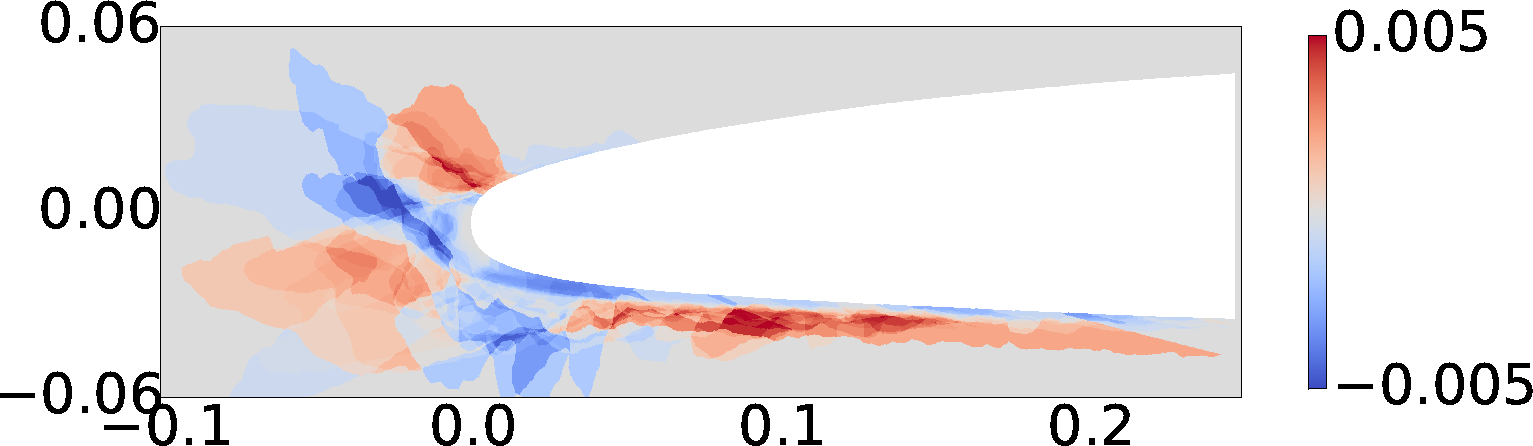
\includegraphics[width=1\textwidth]{MODE5.png} \\
    {\bf Mode 5}
\end{columns}

\begin{itemize}
\item \textbf{Model using POD}
\end{itemize}
\begin{equation*}
I(\bv{x}) = \overbar{I(\bv{x})} + \sum_{i=1}^M c_i \Phi_i(\bv{x})
\end{equation*}
\end{frame}
\begin{frame}
\frametitle{Previous Work: Data-Driven UQ}
\label{sec-1-6}

\begin{figure}
  \centering
  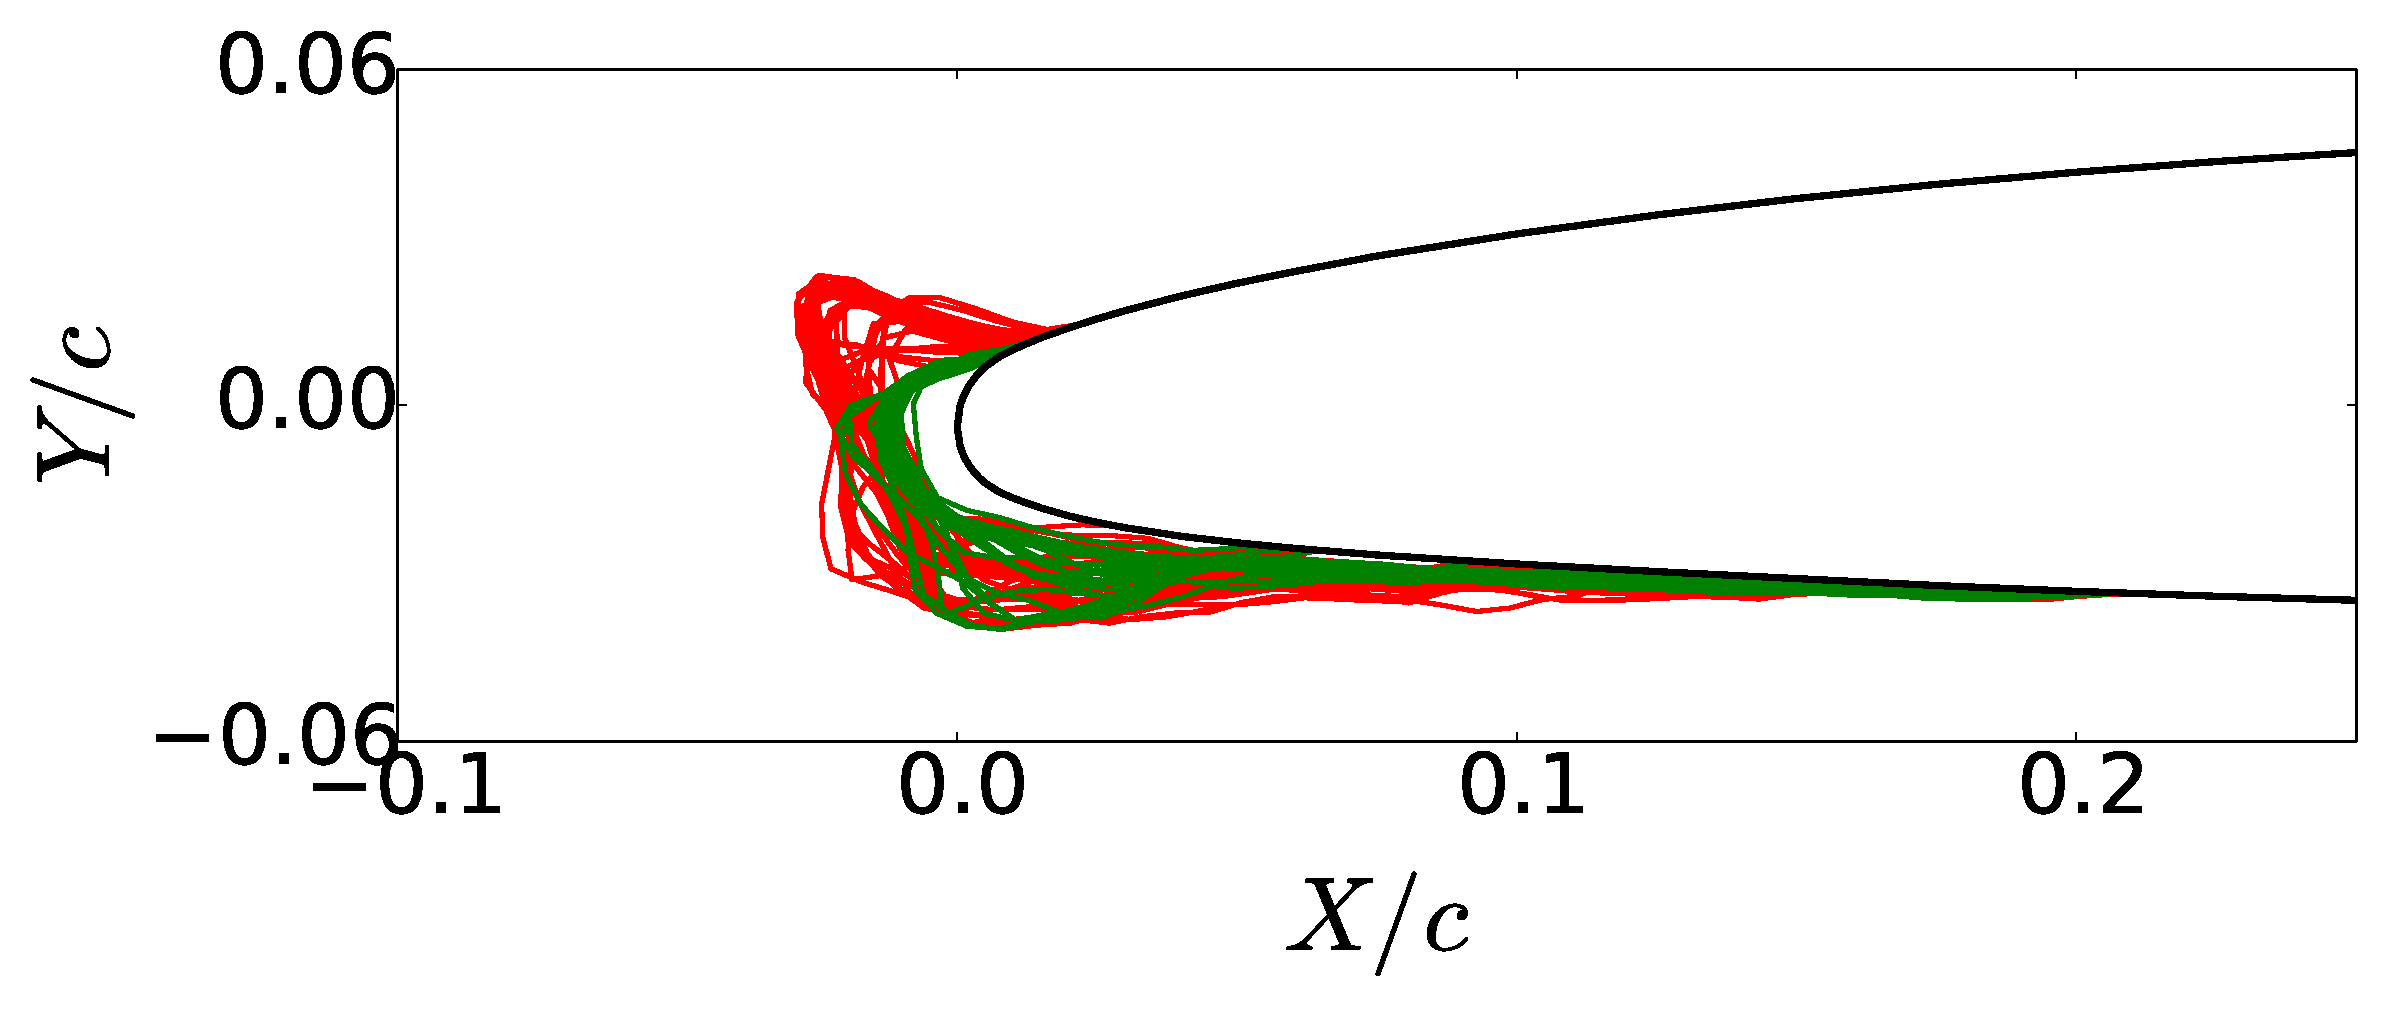
\includegraphics[width=0.7\textwidth]{GoodBadHornExamps}
\end{figure}

\begin{itemize}
\item \textbf{Analyze statistical trends} \footnote{DeGennaro A., Rowley C.W., and Martinelli
L. \emph{Data-Driven Low-Dimensional Modeling and Uncertainty Quantification for Airfoil Icing}. AIAA 2015-3383.
 }
\begin{itemize}
\item Most/least ``harmful'' model shapes are red/green above
\item Quantify aerodynamic performance metric PDFs given input PDF on
    POD parameter space
\item Correlate different input parameters with aerodynamic performance
\end{itemize}
\end{itemize}
\end{frame}
\section{Computational-Based UQ}
\label{sec-2}
\begin{frame}
\frametitle{Motivation}
\label{sec-2-1}

\begin{itemize}
\item \textbf{Investigate uncertainty in the physical process of icing}
\begin{itemize}
\item Droplet diameter distribution
\begin{itemize}
\item Affects collection efficiency
\end{itemize}
\item Droplet temperature distribution
\begin{itemize}
\item Affects convective heat transfer
\item Affects surface tension --> surface roughness
\end{itemize}
\item Surface roughness
\begin{itemize}
\item Can affect local convective heat transfer
\item Can influence local rate of ice accretion
\end{itemize}
\end{itemize}
\end{itemize}
\end{frame}
\begin{frame}
\frametitle{Droplet Diameter Distribution}
\label{sec-2-2}

\begin{columns}[c]
  \column{0.5\textwidth}
    \centering
    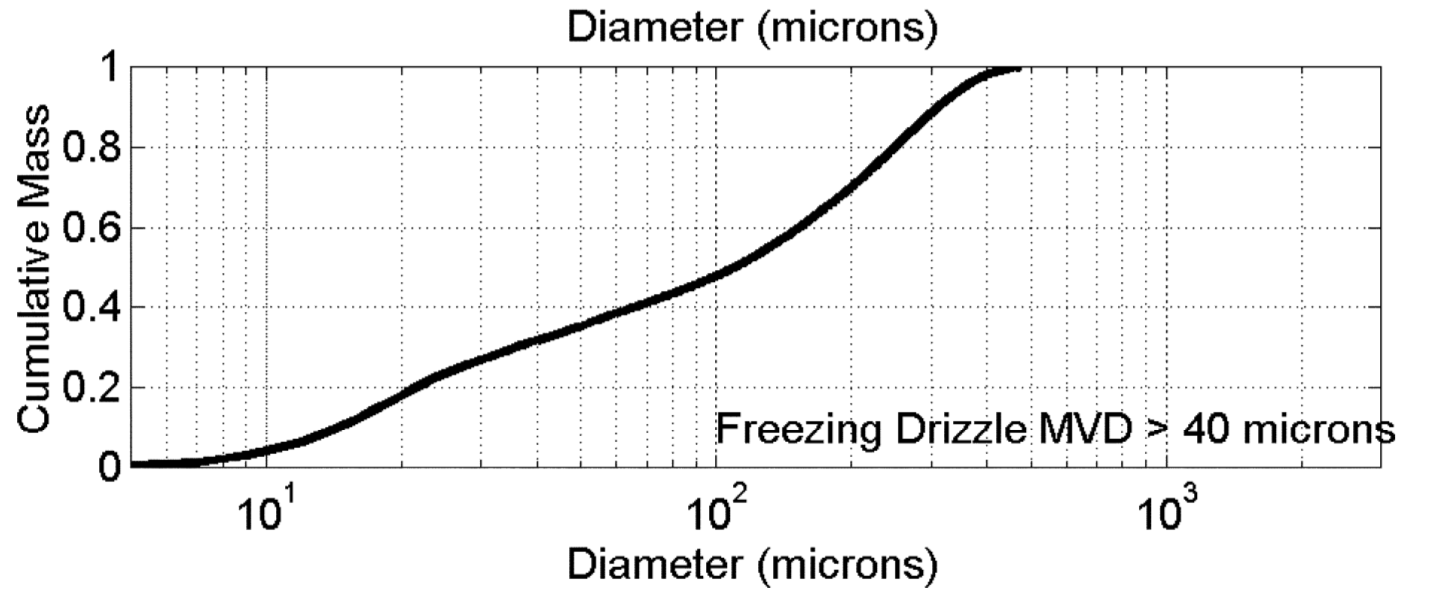
\includegraphics[width=1\textwidth]{FAADropletDist1} \\
    {\bf Freezing Drizzle MVD PDF}
  \column{0.5\textwidth}
    \centering
    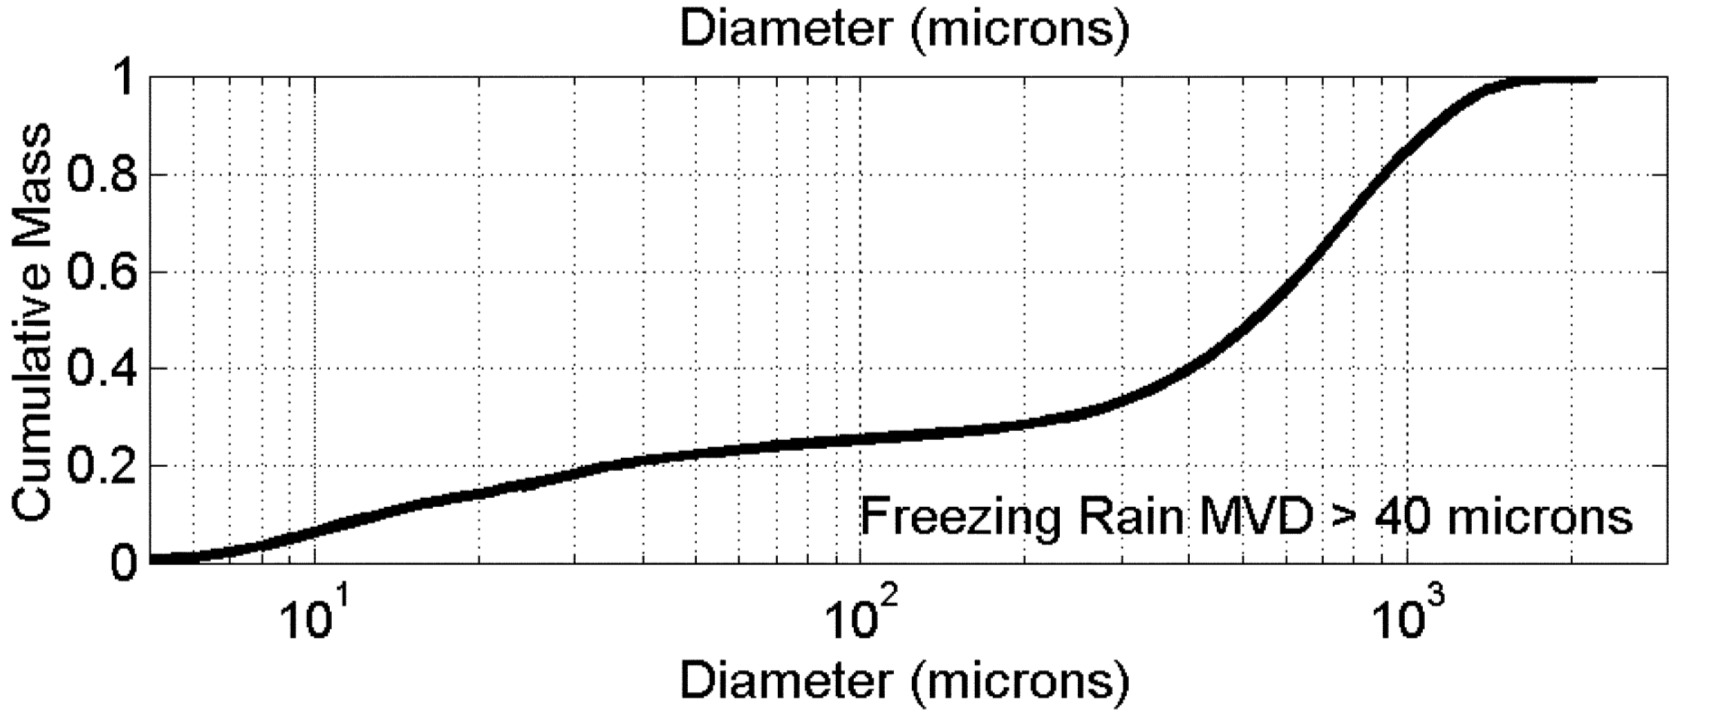
\includegraphics[width=1\textwidth]{FAADropletDist2} \\
    {\bf Freezing Rain MVD PDF}
\end{columns}

\begin{itemize}
\item Several MVD distributions exist for different flight conditions \footnote{Airplane and Engine Certification Requirements in
Supercooled Large Drop, Mixed Phase, and Ice Crystal Icing Conditions;
Final Rule. Federal Register, Vol. 79, No. 213.
 }
\item Each gives a different collection efficiency
\item How sensitive are collection efficiency and ice shape to perturbations in MVD distribution?
\end{itemize}
\end{frame}
\begin{frame}
\frametitle{Surface Tension vs. Temperature}
\label{sec-2-3}

\begin{figure}
  \centering
  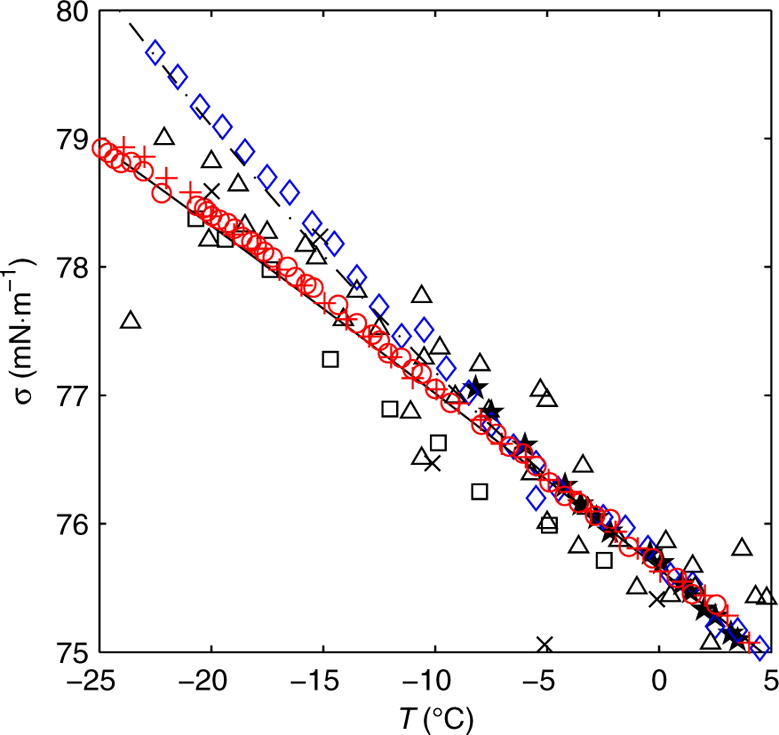
\includegraphics[width=0.33\textwidth]{SurfaceTensionVsTemp.jpeg} \\
  {\bf Surface Tension vs. Temperature}
\end{figure}

\begin{itemize}
\item Surface tension of SLDs varies with temperature \footnote{Hruby, J. et. al. Surface Tension of Supercooled Water:
No Inflection Point down -25 Degrees
Celsius. J. Phys. Chem. Lett. 2014, 5, 425-28.
 }
\item Varying surface tension can affect collection efficiency
\item Higher surface tension may give rise to ``beading'' on surface
  (vs. deposition into film), which could affect surface roughness
\end{itemize}
\end{frame}
\begin{frame}
\frametitle{Roughness Variations}
\label{sec-2-4}

\begin{figure}
  \centering
  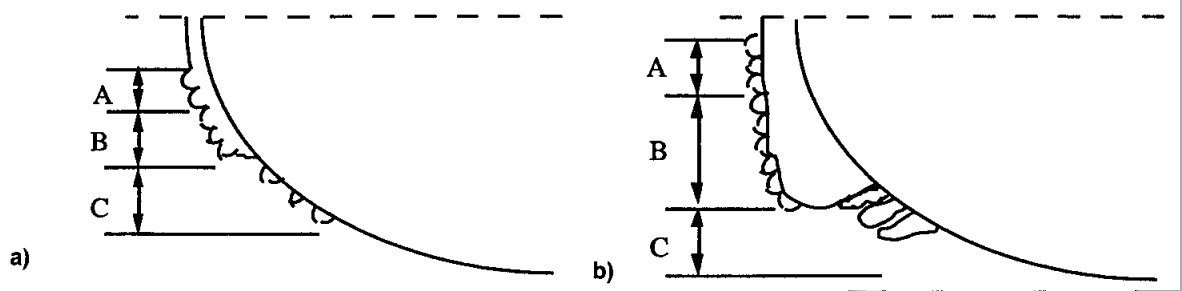
\includegraphics[width=1\textwidth]{IcingRoughness.png} \\
  {\bf Roughness Growth}
\end{figure}

\begin{itemize}
\item \textbf{Surface roughness varies with parameters} \footnote{Shin, J. Characteristics of Surface Roughness Associated
with Leading-Edge Ice Accretion. Journal of Aircraft, Vol. 33, No.2,
April 1996.
 }
\begin{itemize}
\item Roughness height increases with temperature and LWC
\item Beginning of roughness varies with temperature, speed, LWC
\end{itemize}
\item \textbf{Surface roughness affects shape/aerodynamics} \footnotemark[8]
\begin{itemize}
\item Roughness elements probably protrude out of boundary layer and cause transition
\item Irregularity of shape should be calculated by ice accretion code, not treated as part of roughness model
\end{itemize}
\end{itemize}
\end{frame}
\begin{frame}
\frametitle{Airfoil Icing Code Flowchart}
\label{sec-2-5}


\fontsize{7}\selectfont
% Define the layers to draw the diagram
\pgfdeclarelayer{background}
\pgfdeclarelayer{foreground}
\pgfsetlayers{background,main,foreground}

% Define block styles used later

\tikzstyle{sensor}=[draw, fill=blue!20, text width=5em, 
    text centered, minimum height=2.5em,drop shadow]
\tikzstyle{ann} = [above, text width=5em, text centered]
\tikzstyle{wa} = [sensor, text width=7.5em, fill=blue!20, 
    minimum height=3em, rounded corners, drop shadow]

% Define distances for bordering
\def\blockdist{2.3}
\def\edgedist{2.5}

\begin{tikzpicture}
    \node (CleanAirfoil) [wa]  {Clean Airfoil Geometry};
    \path (CleanAirfoil)+(4,2.5) node (FlowSolver) [wa] {Mesh/Flow Solver};
    \path (FlowSolver)+(0,-1.25) node (Droplet) [wa] {Droplet\\Advection Module};
    \path (Droplet)+(0,-1.25) node (ThermoModule) [wa] {Thermodynamic Module};
    \path (ThermoModule)+(0,-1.25) node (IcedAirfoil) [wa] {Iced Airfoil Geometry};
    \path (CleanAirfoil)+(8,0) node (FinalAirfoil) [wa] {Final Iced Airfoil Geometry};

    \path [draw, ->, thick] (CleanAirfoil.north) |- node [above] {} (FlowSolver.west);
    \path [draw, ->, thick] (FlowSolver.south) -- node [below] {} (Droplet.north);
    \path [draw, ->, thick] (Droplet.south) -- node [below] {} (ThermoModule.north);
    \path [draw, ->, thick] (ThermoModule.south) -- node [below] {} (IcedAirfoil.north);
    \path [draw, ->, thick] (IcedAirfoil.east) -| node [above] {} (FinalAirfoil.south);
    \path [draw, ->, thick] (IcedAirfoil.east) -- ++(0.75,0cm) |- node [above]
                      {} (FlowSolver.east);

    \begin{pgfonlayer}{background}
        \path (FlowSolver.west)+(-1,1) node (a) {};
        \path (IcedAirfoil.east)+(1,-1) node (b) {};
        \path[fill=orange!20,rounded corners, draw=black!50, dashed] (a) rectangle (b);
            
    \end{pgfonlayer}

\end{tikzpicture}
\end{frame}
\begin{frame}
\frametitle{Airfoil Icing Code Details}
\label{sec-2-6}

\begin{itemize}
\item \textbf{Droplet advection}
\begin{itemize}
\item Lagrangian formulation of equations of motion
\item Impingement details depend on ratio of inertial to viscous forces
\begin{itemize}
\item Impacting droplets can bounce, deposit into surface film, or splash
\end{itemize}
\item Ratio of local to free-stream flux of droplets is calculated over airfoil
\end{itemize}
\item \textbf{Thermodynamics}
\begin{itemize}
\item Mass and energy balances of the liquid film on the airfoil surface
    used to determine ice accretion on airfoil
\item Mass enters film through impinging droplets, exits by freezing
\item Energy enters/exits through internal/kinetic energy of impinging
    droplets, energy transfer by ice accretion, convective
    heat transfer between ice/film/wall and the flow
\item Coupled mass/energy PDEs can be solved in one of two ways: (1)
    ``elephant gun'': Jacobian-free Newton-Krylov (JFNK) iteration, or
    (2) guess solution, drive to steady-state
\end{itemize}
\end{itemize}
\end{frame}
\begin{frame}
\frametitle{State of Code: Advection Module}
\label{sec-2-7}


\begin{columns}[c]
  \column{0.5\textwidth}
    \centering
    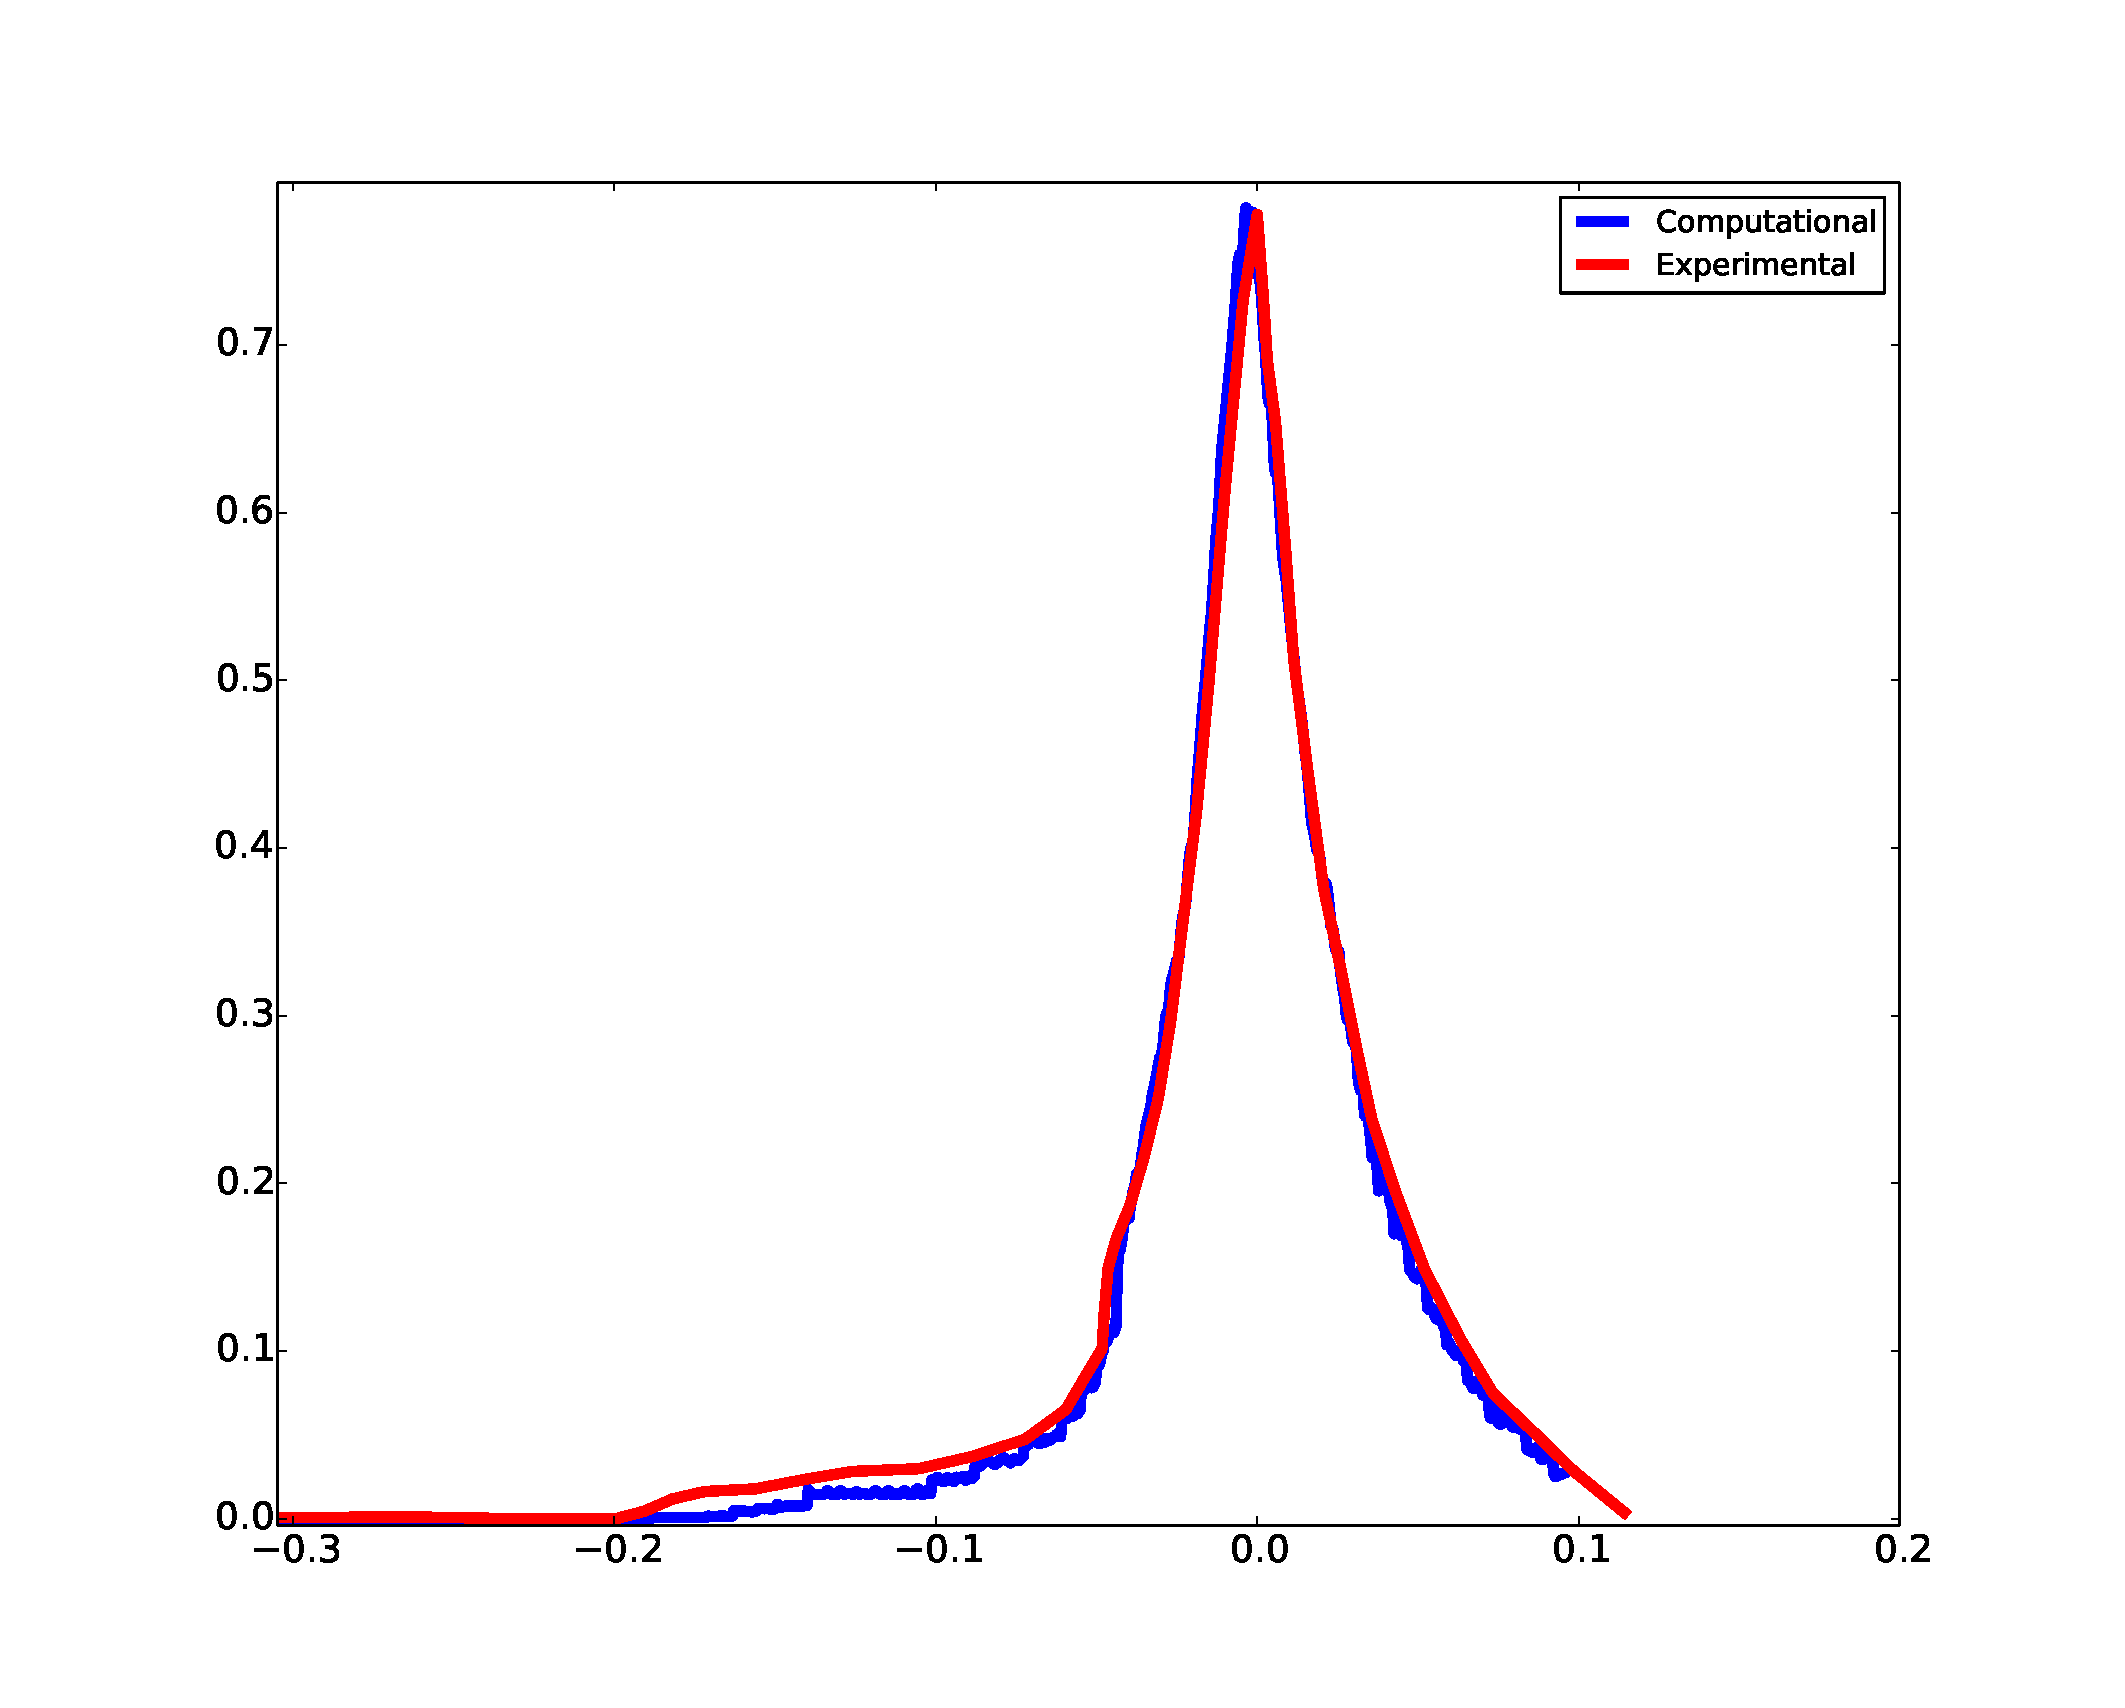
\includegraphics[width=0.65\textwidth]{MVD52} \\
    {\bf MVD 52} \\
    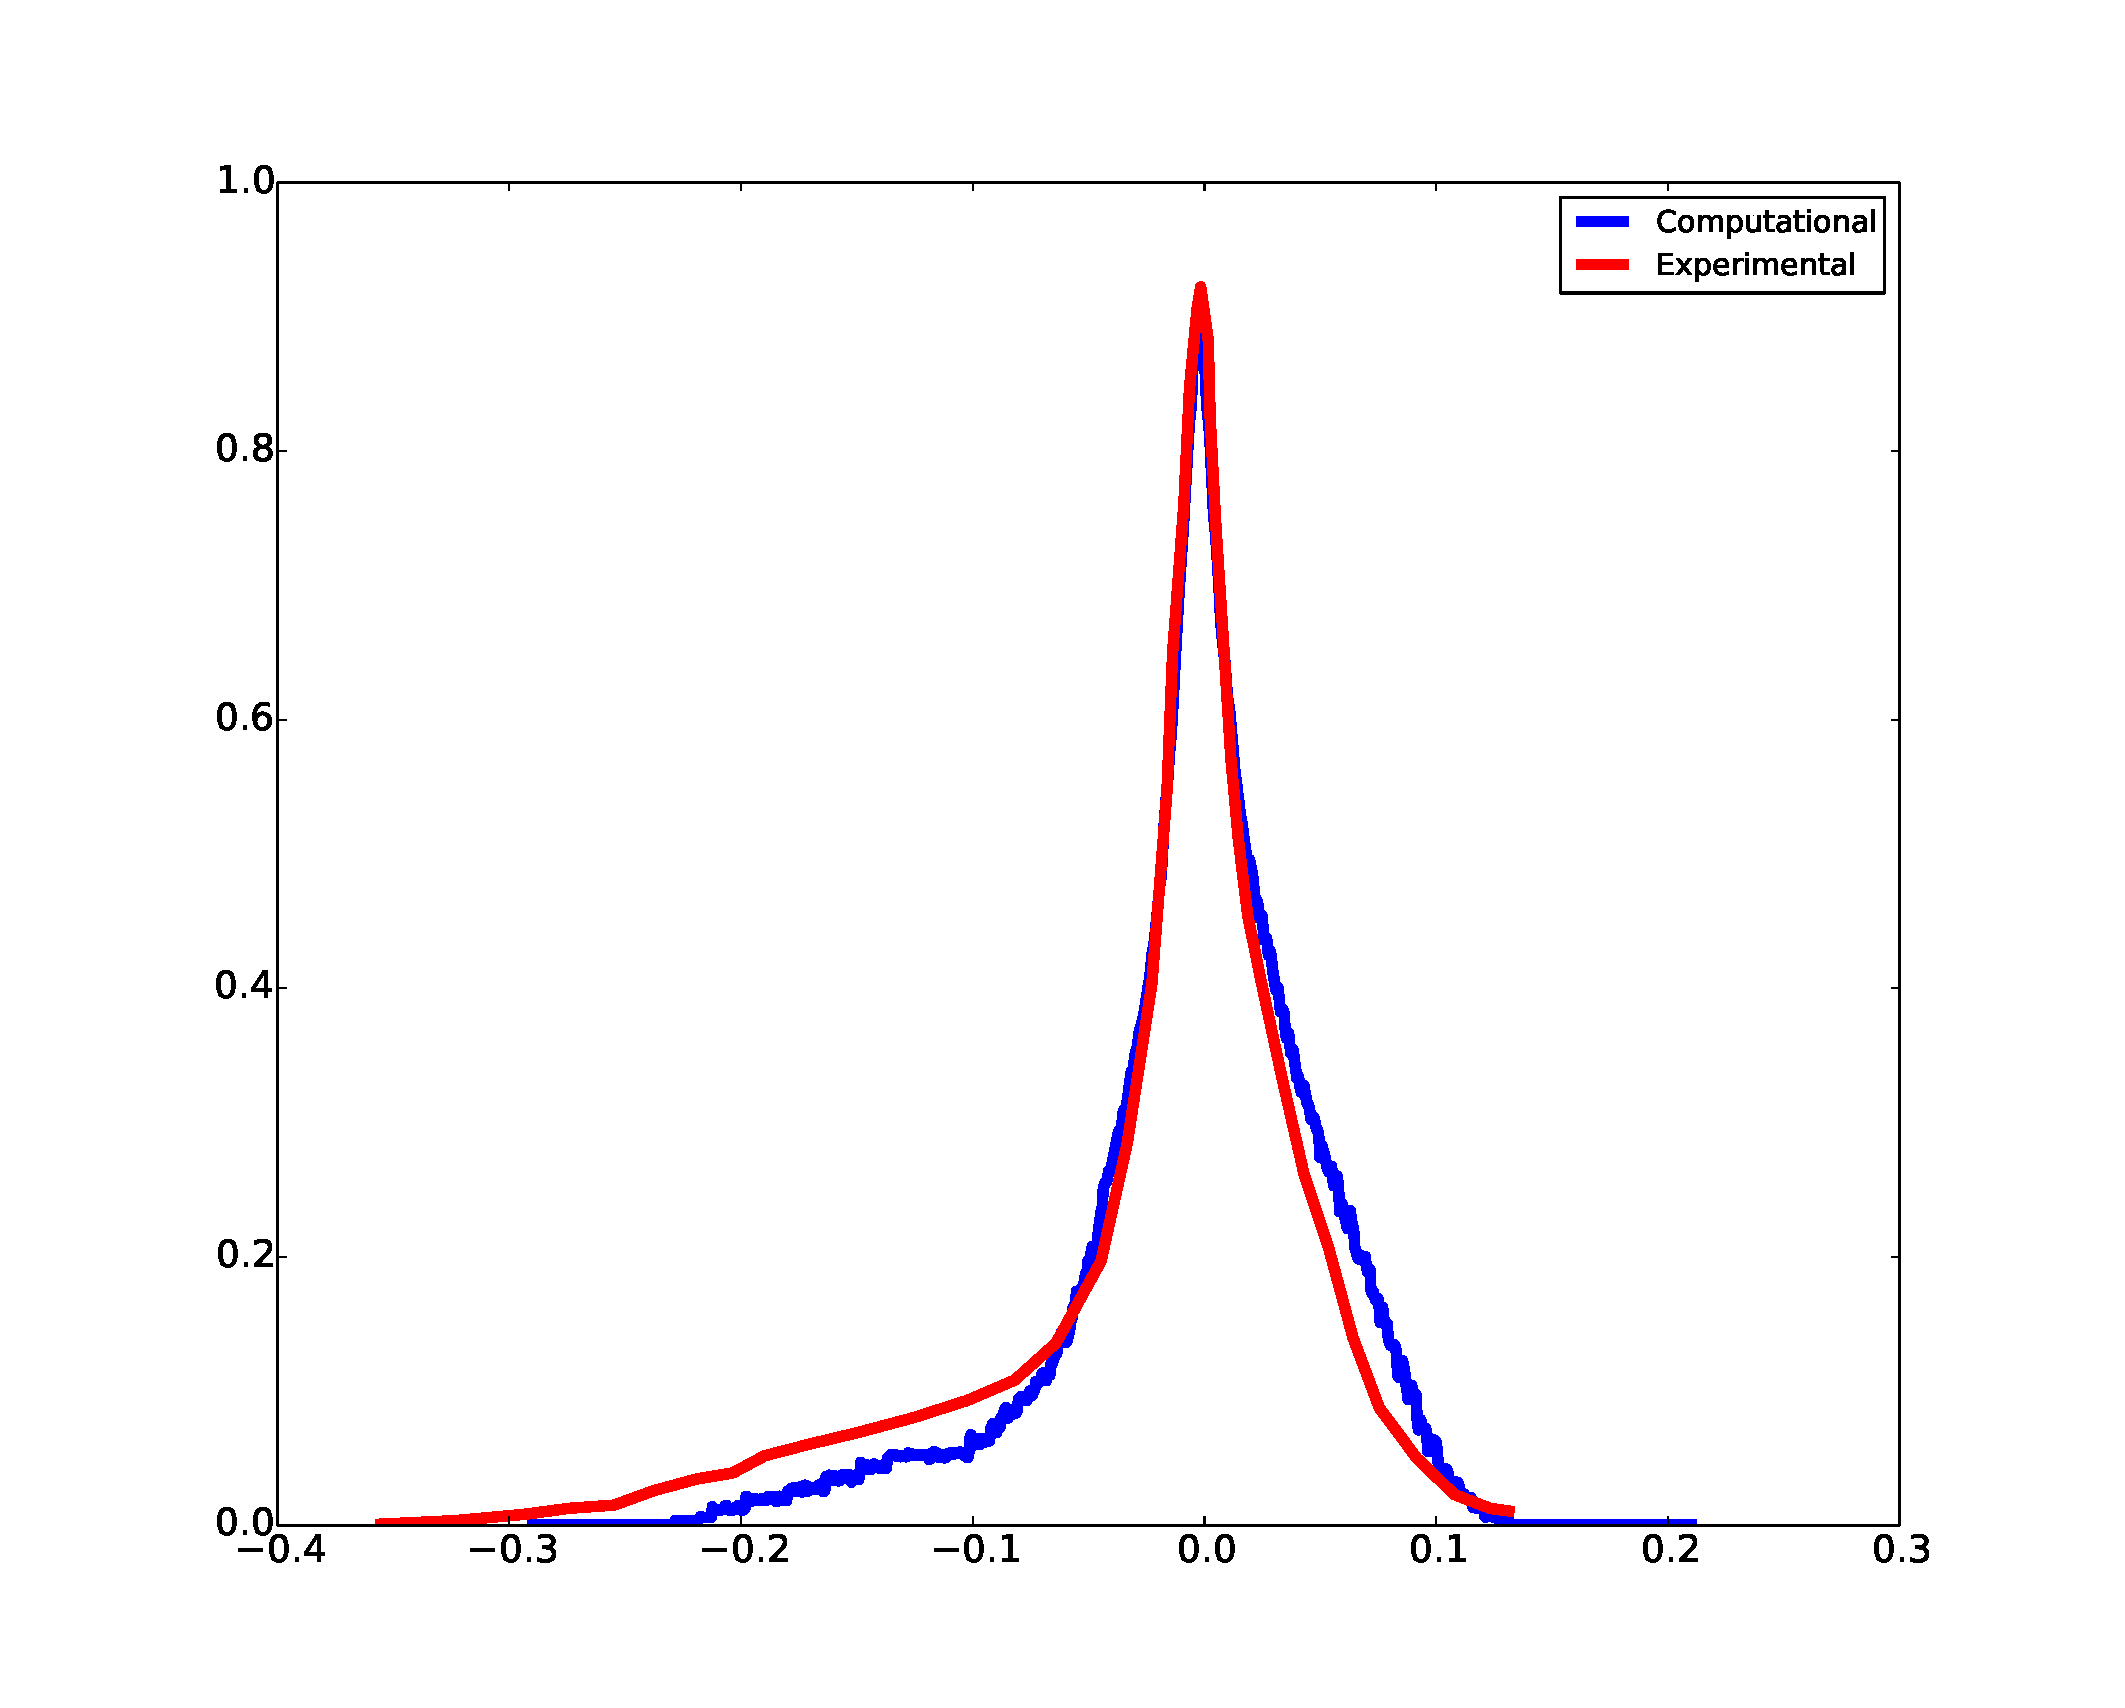
\includegraphics[width=0.65\textwidth]{MVD154} \\
    {\bf MVD 154}
  \column{0.5\textwidth}
    \centering
    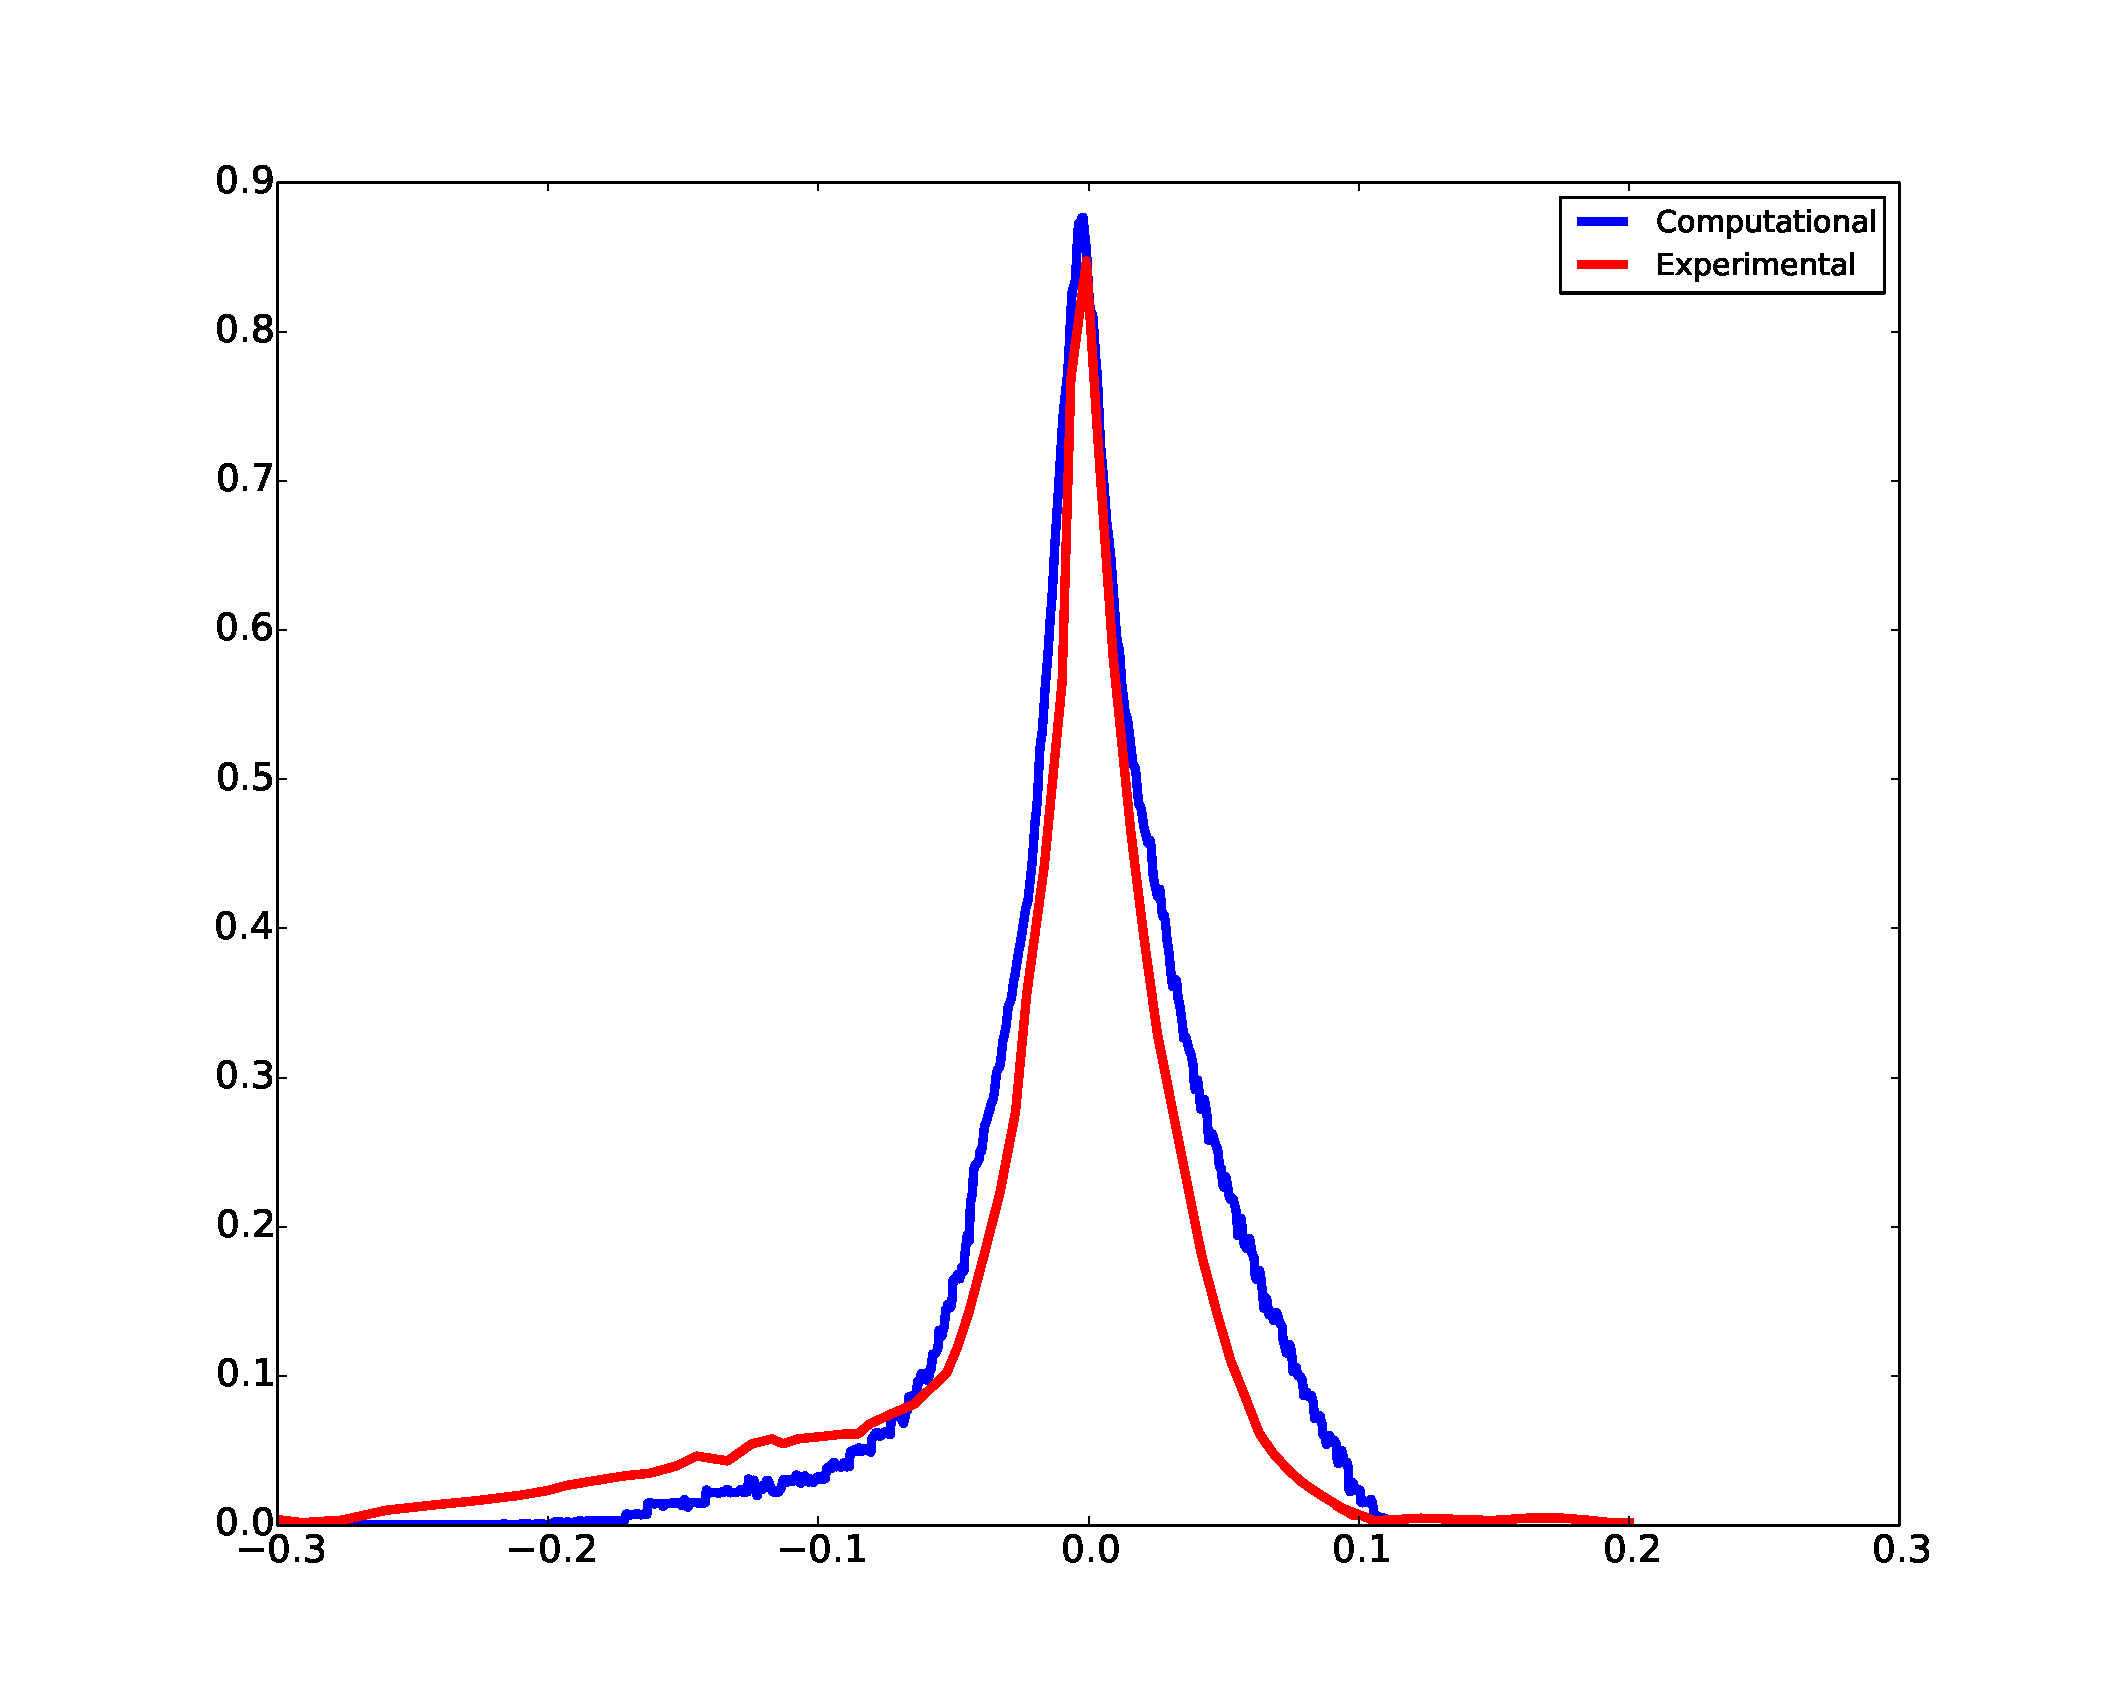
\includegraphics[width=0.65\textwidth]{MVD111} \\
    {\bf MVD 111} \\
    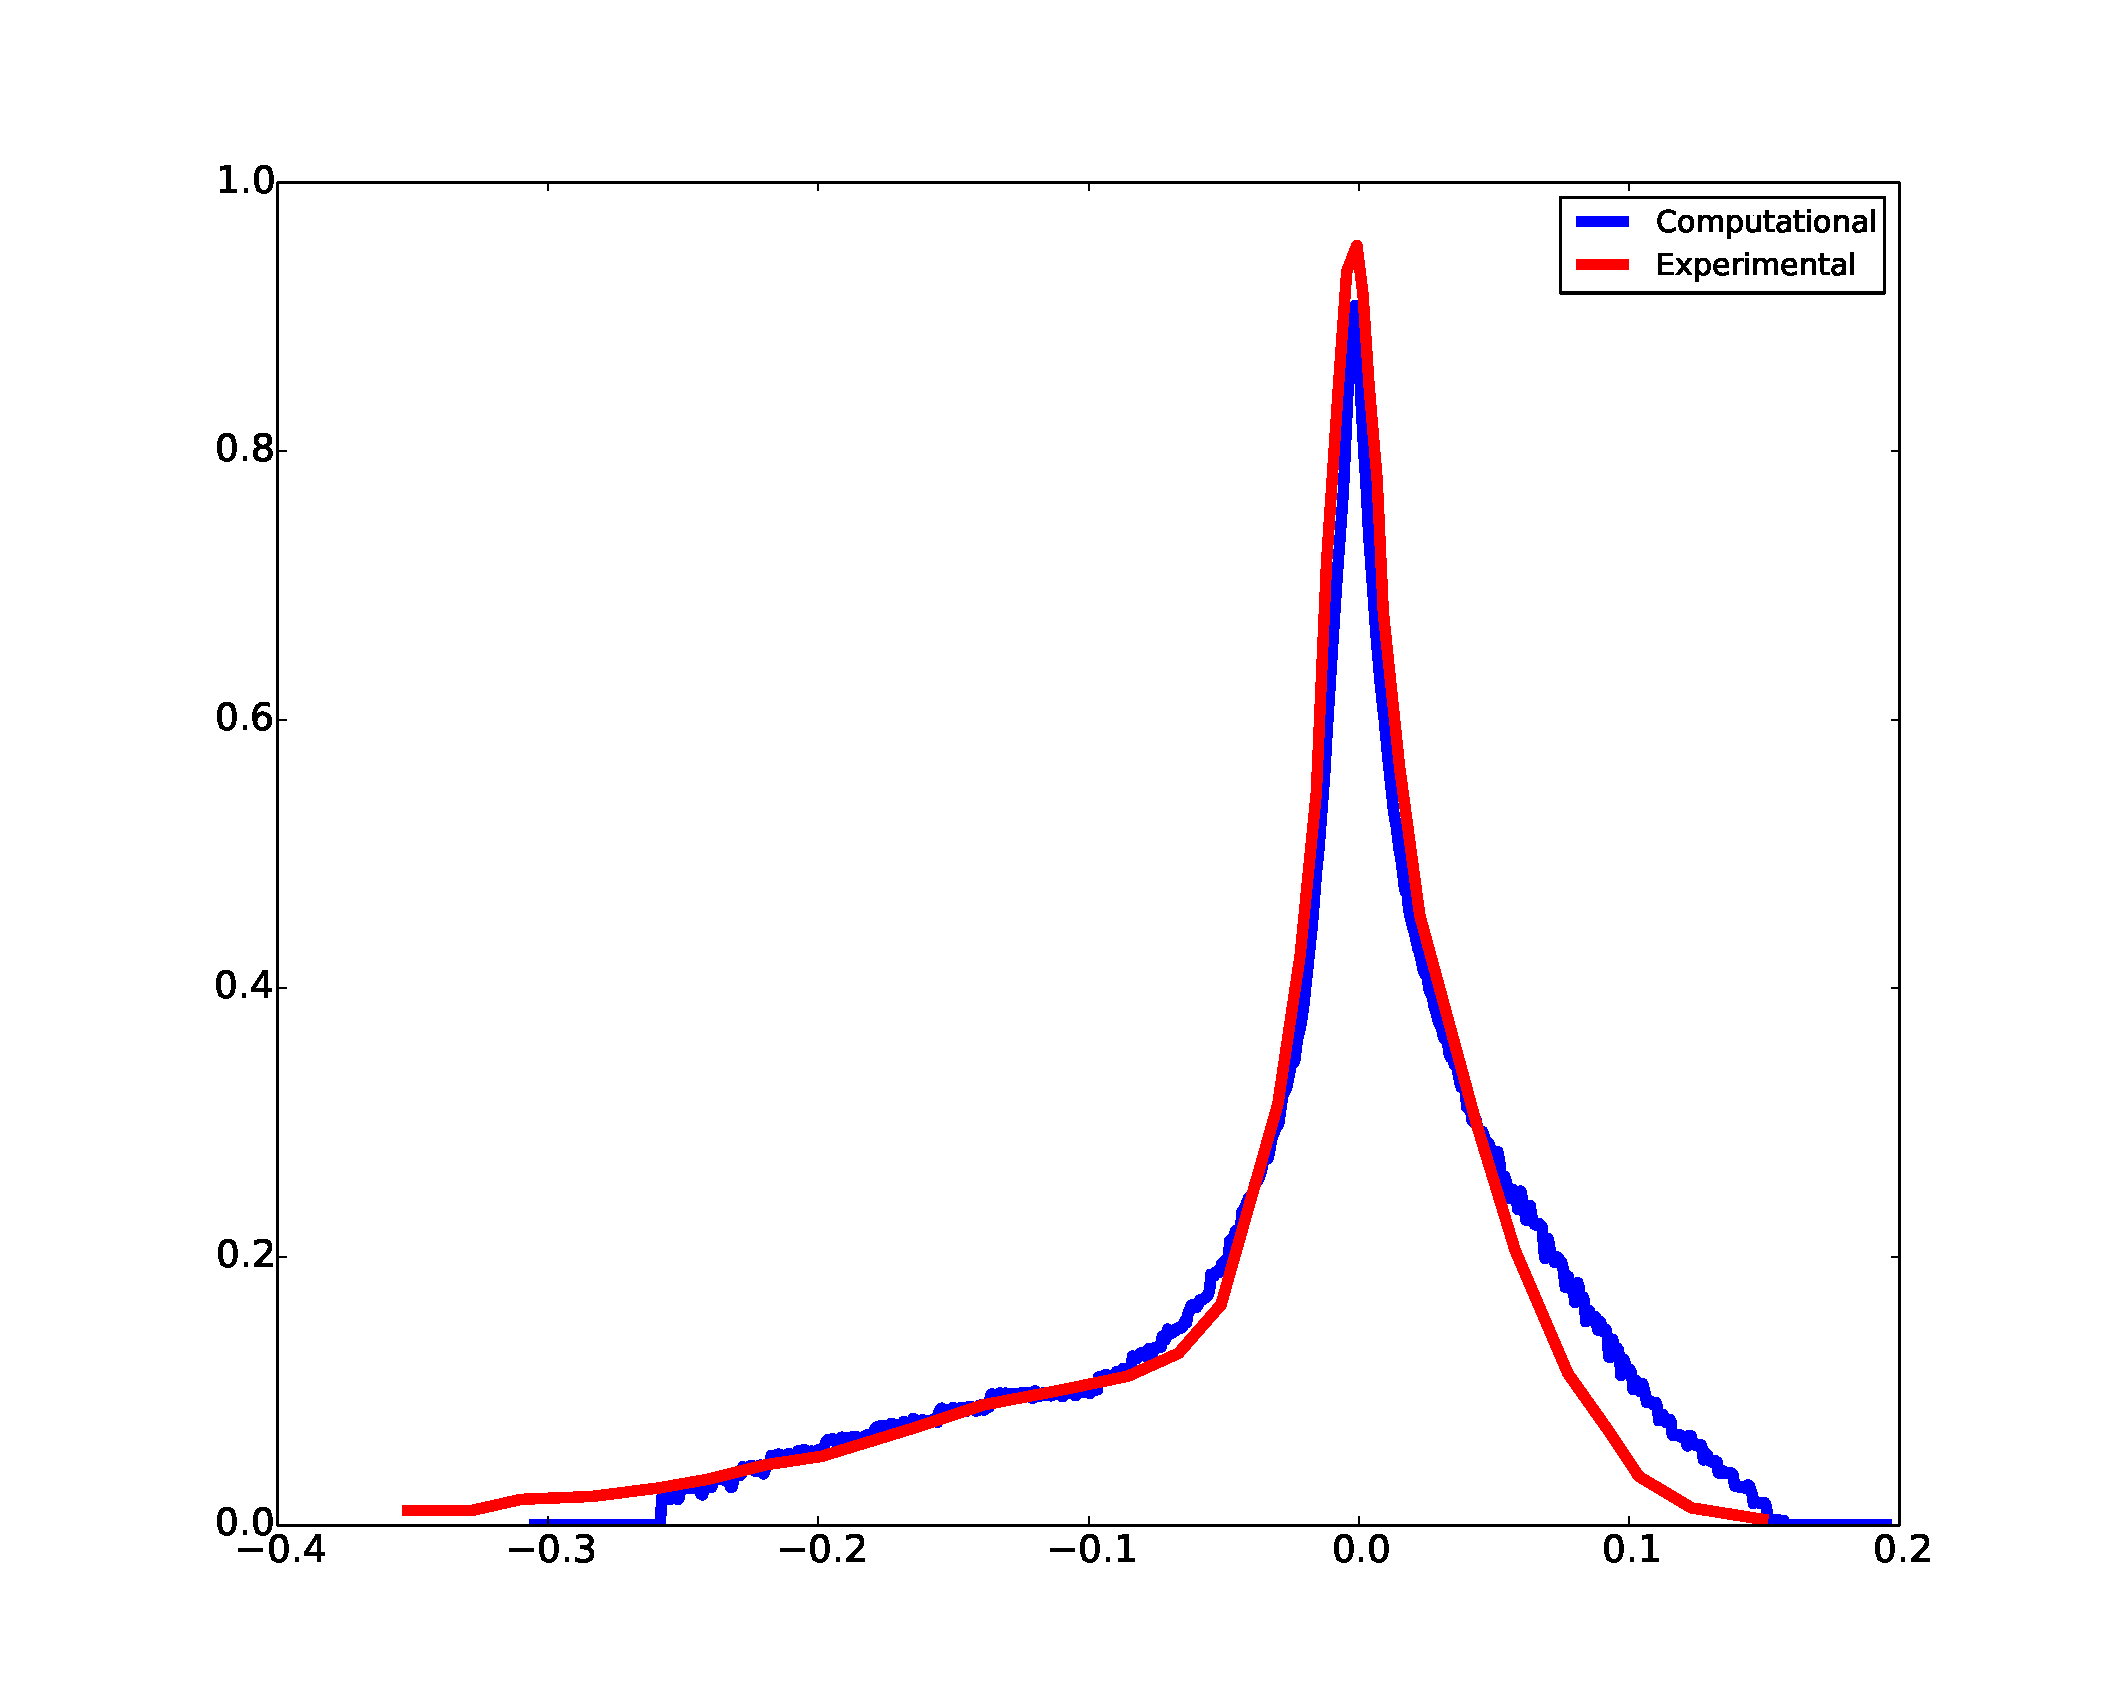
\includegraphics[width=0.65\textwidth]{MVD236} \\
    {\bf MVD 236}
\end{columns}

\begin{itemize}
\item Advection module appears to be giving reasonable results for
  benchmark tests using different droplet distributions on a clean
  airfoil
\end{itemize}
\end{frame}
\begin{frame}
\frametitle{State of Code: Thermodynamic Module}
\label{sec-2-8}

\begin{itemize}
\item \textbf{Completed work}
\begin{itemize}
\item Finite volume discretization of the mass/energy equations with
    appropriate upwinding (Roe scheme)
\item Modifications to Gigi's flow solver to compute/output convective
    heat transfer coefficient, skin friction
\item Basic MatLab prototyping for solving equations with (1) JFNK and (2)
    explicitly driving initial guess to steady-state
\end{itemize}
\item \textbf{Remaining work}
\begin{itemize}
\item Modify Spalart-Almaras turbulence model in flow solver for rough
    wall/icing application (will affect convective heat transfer)
\item Integrate MatLab prototype solver into main C++ icing code
\item Test, verify calculations!
\item Once working, do UQ studies on physical parameters (eg.,
    convective heat transfer distribution, droplet size and
    temperature distribution) affect aerodynamics
\end{itemize}
\end{itemize}
\end{frame}
\section{UQ for DMD}
\label{sec-3}
\begin{frame}
\frametitle{Motivation}
\label{sec-3-1}

\begin{itemize}
\item DMD models can change with (1) uncertain physical parameters, or (2) sensor noise
\item Viewing this as a UQ problem has some potential advantages:
\begin{itemize}
\item Some UQ tools can be computationally efficient relative to Monte Carlo sampling
\item Can investigate sensitivity of DMD models to different parameters
\item Can investigate sensitivity of DMD models to noise bias/scaling
\item Can assemble a surrogate model for how DMD models change over a parameter range
\end{itemize}
\end{itemize}
\end{frame}
\begin{frame}
\frametitle{Basic Demonstration: Parametric Uncertainty}
\label{sec-3-2}

\begin{itemize}
\item Stuart-Landau equation, $\mu = \mathcal{U}(1,1.2)$, $\beta = \mathcal{U}(0,0.2)$
\end{itemize}
\begin{equation*}
\begin{aligned}
\dot{r} &= \mu r - r^3 \\
\dot{\theta} &= \gamma - \beta r^2
\end{aligned}
\end{equation*}
\begin{itemize}
\item Observations are $\lbrace r^{-j} e^{i(k\theta)} \rbrace$, $j = -2,0$ and $k = -3...3$
\end{itemize}

\begin{columns}[c]
  \column{0.5\textwidth}
    \centering
    \includegraphics[width=0.99\textwidth]{SLeigs_PCE} \\
    {\bf PCE Evalss (129 Samples)}
  \column{0.5\textwidth}
    \centering
    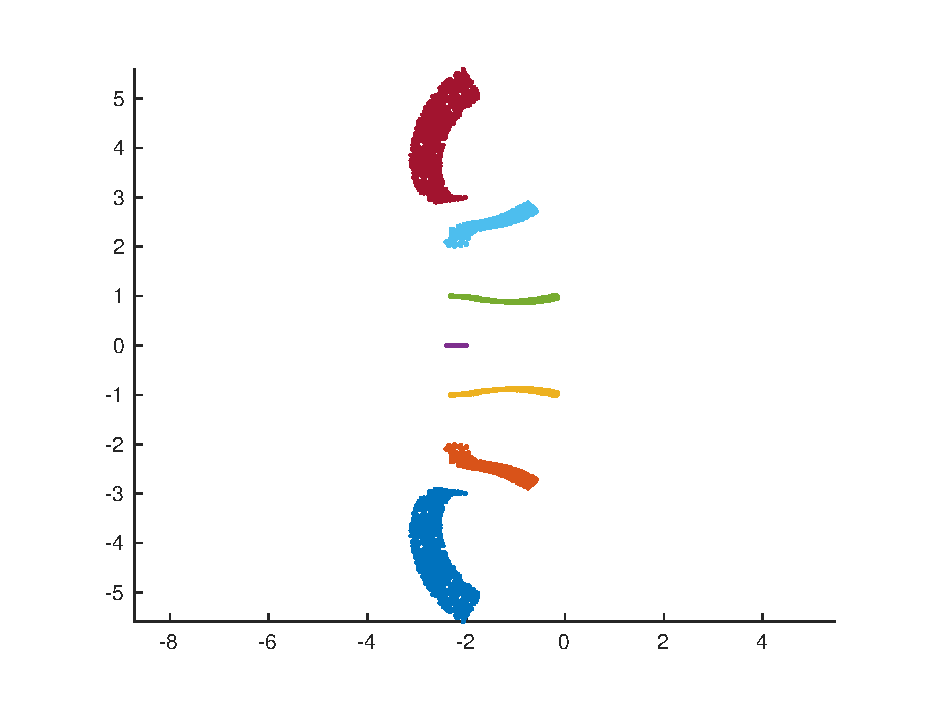
\includegraphics[width=0.99\textwidth]{SLeigs_MC} \\
    {\bf Monte Carlo Evals (1000 Samples)}
\end{columns}
\end{frame}
\begin{frame}
\frametitle{Basic Demonstration: Noise-Corrupted Data}
\label{sec-3-3}

\newcommand*{\horzbar}{\rule[.5ex]{2.5ex}{0.5pt}}
\begin{equation*}
\dot{\bv{x}} =  \begin{bmatrix} 1 & -2 \\ 1 & -1 \end{bmatrix} \bv{x}
\end{equation*}

\begin{itemize}
\item Take data $X \in \mathbb{R}^{2\times100}$ as 100 discrete-time samples of system ($dt = 0.1$)
\item Data is corrupted by noise matrix $N \in \mathbb{R}^{2\times100}$
\end{itemize}

\begin{equation*}
N = \begin{bmatrix} \horzbar & N_1(\mu_1,\sigma_1) & \horzbar \\ \horzbar & N_2(\mu_2,\sigma_2) & \horzbar \end{bmatrix}
\end{equation*}

\begin{columns}[c]
  \column{0.5\textwidth}
    \centering
    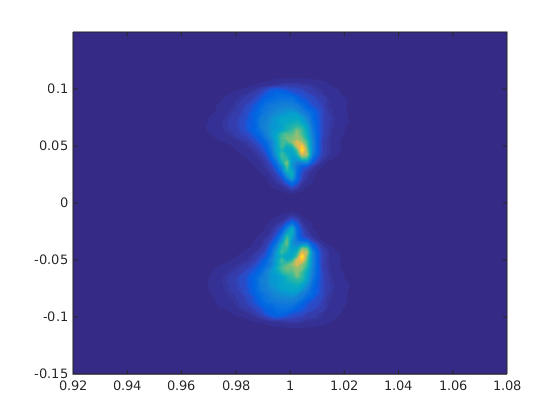
\includegraphics[width=0.75\textwidth]{NoisyEigsPCE} \\
    {\bf PCE Evals (337 Samples)}
  \column{0.5\textwidth}
    \centering
    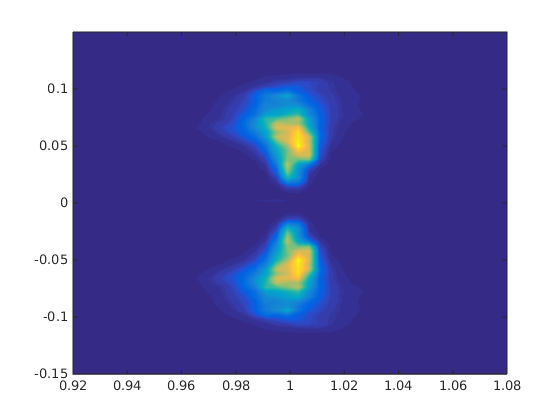
\includegraphics[width=0.75\textwidth]{NoisyEigsMC} \\
    {\bf Monte Carlo Evals (1000 Samples)}
\end{columns}
\end{frame}
\begin{frame}
\frametitle{Future Work}
\label{sec-3-4}

\begin{itemize}
\item Extending work to ``realistic'' cases where the state dimension is large
\end{itemize}
\end{frame}

\end{document}
